%
\def\year{2018}\relax
\documentclass[letterpaper]{article} %DO NOT CHANGE THIS
\newcounter{bab}
\renewcommand{\thebab}{The Bounded Alpha-Beta Algorithm}

\usepackage{aaai18}  %Required
\usepackage{times}  %Required
\usepackage{helvet}  %Required
\usepackage{courier}  %Required
\usepackage{url}  %Required
\usepackage{graphicx}  %Required
\usepackage{subfig}
\usepackage{soul}


\usepackage{tikz}
\usetikzlibrary{arrows,shapes,positioning,mindmap,calc}
\tikzset{style={>=stealth'}}
\tikzset{minnode/.style={align=left,font=\footnotesize,circle,    fill=white,draw=black, minimum size=7mm,inner sep=1mm}}
\tikzset{maxnode/.style={align=left,font=\footnotesize,rectangle,fill=white,draw=black,  minimum size=6mm,inner sep=1mm}}
%\tikzset{targetk/.style={star,     fill=white,draw=red,  text=red,  minimum size=8mm,inner sep=0mm}}
\tikzset{infobox/.style={align=left,font=\footnotesize,minimum size=6mm}}

\frenchspacing  %Required
\setlength{\pdfpagewidth}{8.5in}  %Required
\setlength{\pdfpageheight}{11in}  %Required

\usepackage[ruled,vlined,linesnumbered]{algorithm2e}
\usepackage{amsmath}
\usepackage{amsthm}
\usepackage{url}
\usepackage{multirow}

%PDF Info Is Required:
  \pdfinfo{
/Title (Bounded Suboptimal Game Tree Search)
/Author (Dor Atzmon, Roni Stern, Abdallah Saffidine)}
\setcounter{secnumdepth}{0} 


\newtheorem{definition}{Definition}
\newtheorem{lemma}{Lemma}
\newtheorem{theorem}{Theorem}
\newcommand{\ignore}[1]{}
%\newcommand{\pess}{\mathit{pess}}
%\newcommand{\opti}{\mathit{opti}}
\newcommand{\MM}{\mathit{V}}
\newcommand{\pess}{\mathit{L}}
\newcommand{\opti}{\mathit{U}}
\newcommand{\besto}{\mathit{best}_{\opti}}
\newcommand{\bestp}{\mathit{best}_{\pess}}
\newcommand{\eval}{\mathit{eval}}
\newcommand{\bab}{\mathit{BAB}}
\newcommand{\vmax}{v_{\text{max}}}
\newcommand{\vmin}{v_{\text{min}}}
\newcommand{\rootnode}{\mathit{n_1}}
\newcommand{\amb}{\textit{AMB}}
\newcommand{\er}{\textit{ER}}
\newcommand{\tuple}[1]{\langle #1 \rangle}
% correct bad hyphenation here


\begin{document}
\title{Bounded Suboptimal Game Tree Search}
\author{Dor Atzmon \and Roni Stern\\
Ben Gurion University of the Negev\\
Be'er Sheva, Israel
\And
Abdallah Saffidine \\
Australian National University\\
Canberra, Australia}

\maketitle

% As a general rule, do not put math, special symbols or citations
% in the abstract
\begin{abstract}
Finding the minimax value of a game is an important problem in a variety of fields, including game theory, decision theory,  statistics, philosophy, economics, robotics, and security. Classical algorithms such as the Minimax algorithm can be used to find the minimax value, but require iterating over the entire game tree, which is in many cases too large. Alpha-Beta pruning identifies portions of the game tree that are not necessary for finding the minimax value, but in many cases the remaining part of the game tree is still too large to search in reasonable time. For such cases, we propose a class of algorithms that accepts a parameter $\epsilon$ and returns a value that is guaranteed to be at most $\epsilon$ away from the true minimax value. We lay the theoretical foundation for building such algorithms and present one such algorithm based on Alpha-Beta. Experimentally, we show that our  algorithm allows controlling this runtime/solution quality tradeoff effectively. %  is able to do significantly more pruning than Alpha-Beta as a function of the given $\epsilon$, demonstrating the desired tradeoff in practice. 


%Such ``bounded-suboptimal'' game tree search algorithms provide a mechanism for controlling trading solution quality for runtime ``bounded-suboptimal'' approach:  To this end, we propose a general method for finding approximately  For such cases, we propose a bounded-suboptimal approach for finding the minimax value, in which we return a value that is close to the real minimax value by performing this work, we provide a mechanism for controlling trading solution quality for runtime, this tradeoff: a family of bounded-minimax algorithms, which are algorithms that  accept a parameter $\epsilon$ and return a range around the minimax value instead of the exact value, where the size of this range is bounded by $\epsilon$. %These algorithms can prune larger portions of the game tree and thus be faster than minimax with Alpha-Beta pruning, providing a natural tradeoff between solution quality and runtime. 

%general pruning rules that provide a mechanism for controlling this trade-off, specifying exactly how a parameter $\epsilon$ that 
%can prune larger portions of the game tree than Alpha-Beta pruning by allowing it to return a bounding range around the minimax value instead of the exact minimax value. The size of this range is set a-priori by a parameter $\epsilon$, which provides a control over the runtime 
%Finding the minimax value can be done efficiently by the Alpha-beta pruning algorithm, which is a search algorithm that prunes unpromising branches on the search tree.  In this research we learn and study a novel algorithm, called: Bounded alpha-beta (BAB), for finding a bounded suboptimal minimax value. We prove theoretically that BAB guarantee to return a bounded suboptimal minimax value and show empirically that it doing so while saving computational time. 

%Minimax is a decision rule for maximize the profit or minimize the loss in a worst case scenario. The minimax value had a great impact and still being used in a variety of fields, including: game theory, decision theory,  mathematics, statistics, philosophy, economics, robotics, and security.  Finding the minimax value can be done efficiently by the Alpha-beta pruning algorithm, which is a search algorithm that prunes unpromising branches on the search tree.  In this research we learn and study a novel algorithm, called: Bounded alpha-beta (BAB), for finding a bounded suboptimal minimax value. We prove theoretically that BAB guarantee to return a bounded suboptimal minimax value and show empirically that it doing so while saving computational time. 
\end{abstract}


%---------------------------------------------------------
%---------------------------------------------------------


\section{Introduction}

%Solving zero-sum fully observable games has been studied in a variety of fields, including game theory, decision theory,  statistics, philosophy, economics, robotics, and security. 

Minimax is a fundamental decision-making rule in zero-sum games~\cite{wald1945statistical}, 
% cite: Statistical Decision Functions Which Minimize the Maximum Risk
in which a player chooses an action that maximizes its utility assuming the other player will 
choose the action that will minimize its utility. The \emph{minimax value} of a game is the expected utility for the first player obtained assuming both players follow the minimax rule. 
Finding the \emph{minimax value} of a game is a challenging problem with applications in a variety of fields, including game theory, decision theory,  statistics, philosophy, economics, robotics, and security. 
In fact, when the minimax value of a game is found the game is said to be \emph{solved}~\cite{schaeffer2007checkers,irving2000solving,saffidine2011solving}. 


Consequently, many algorithms have been proposed for finding the minimax value of a game, such as the Minimax algorithm, Alpha-Beta, Proof Number Search~\cite{allis1994proof}, Monte Carlo Tree Search~\cite{coulom2006efficient,kocsis2006bandit,lanctot2013monte}, and others. 
Nonetheless, finding the minimax value of many games is still a challenge due to the size of the game tree they define. 

This complexity challenge also exists when solving hard single-agent search problems, where finding optimal solutions is often not feasible. A popular way to address this in single-agent search is to relax the requirement of finding an optimal solution, and allow returning suboptimal solutions. This often raises a runtime versus solution quality tradeoff. Bounded-suboptimal single-agent search algorithms control this tradeoff with a user-defined parameter that bounds the allowed suboptimality of the returned solution. Weighted A*~\cite{pohl1970heuristic}, Explicit Estimation Search~\cite{thayer2011bounded}, and Dynamic Potential Search~\cite{gilon2016dynamic} are examples of such algorithms. 

In this work, we present a theory for building ``bounded-suboptimal'' algorithms for finding the minimax value of game trees. Such algorithms, which we refer to as \emph{bounded-suboptimal game tree} algorithms, are guaranteed to return a value that is at most $\epsilon$ from the true minimax value, where $\epsilon$ is a user-provided parameter. 


We provide a general theory for extending the well-known Alpha-Beta pruning technique to provide bounded-suboptimal solutions. This includes concrete pruning rules for both deterministic games and games with chance, based on *-Minimax~\cite{ballard1983minimax,hauk2004rediscovering}. These pruning rules can be applied to a wide range of game tree search algorithms. We provide details of a concrete game tree search algorithm that uses these rules, called Bounded Alpha-Beta (BAB). Experimentally, BAB shows that it indeed provides the desired tradeoff of runtime for optimality on two domains. 
While the focus of this work is not on developing a new AI game playing algorithm, we also provide preliminary evidence that suggests the pruning done by a player using bounded-suboptimal search algorithm can be effective also for game-playing. 

%---------------------------------------------------------
%---------------------------------------------------------

%[[TODO: FIX INTRO AND ABSTRACT. MAKE MORE FOCUSED AND REMOVE MINIMAX BOUND DISCUSSION]]

\section{Background}

In this work, we focus on finite, two-player, zero-sum game with chance and perfect information, defined as follows. 
%[[Maybe redundant]]
\begin{definition}[Zero-Sum, Perfect Information Game]
A finite, two-player, zero-sum game with chance and perfect information is defined by a tuple $\tuple{\mathcal{S}, \mathcal{T}, \mathcal{A}, \mathcal{P}, \tau, u, s_1}$, where:
(1) $\mathcal{S}$ is a finite, non-empty, set of states; 
(2) $\mathcal{T}\subseteq \mathcal{S}$ is the set of terminal states; 
(3) $\mathcal{A}$ is a finite, non-empty, set of actions; 
(4) $\mathcal{P}$ is a transition probability function where $\mathcal{P}(s,a,s')$ is the probability of getting to state $s'$ after performing $a$ in state $s$; 
(5) $\tau:\mathcal{S}\rightarrow\{1,2\}$ is a player index function, returning the player whose turn is to act in a given state, 
(6) $u$ is a utility function $u:\mathcal{T}\rightarrow [\vmin,\vmax]$, mapping terminal states to their utility to player 1, where $\vmin$ and $\vmax$ denote the minimum and maximum possible utility; 
and (7) $s_1$ is the initial state. 
\label{def:game-with-chance}
\end{definition}
Hereinafter, we use the term \emph{game} to refer to the type of games defined in Def.~\ref{def:game-with-chance}. A game is called \emph{deterministic} if performing an action on a state can lead to exactly one state, i.e., for every state action pair $(s,a)$ there exists a single state $s'$ for which $\mathcal{P}(s,a,s')=1$. 

%We focus in this work on zero-sum perfect information games, either deterministic of with chance. Deterministic games are a special case of games with chance, and so we define only the latter.


% How a game is played
%We define a player index function $\tau:\mathcal{S}\rightarrow\{1,2\}$ that returns the player whose turn is to act in a given state. Since this is a zero-sum game, player 1 prefers states with higher utility while player 2 prefers states with lower utility. %a state with lhigher utility %the utility of a state to player 2 is the negation of that state's utility to player 1. 
We refer to player 1 and player 2 as the MAX player and the MIN player, respectively.
A game starts with the MAX player ($\tau(s_1)=1$). 
In each step the turn player chooses an action from $\mathcal{A}$ to apply to the current state, generating a new state according to the transition probability function $\mathcal{P}$.
This process continues until a player reaches a terminal state, at which point the MAX player gets the utility of that state. % Text can be improved

% The game tree
A game defines a tree, referred to as the \emph{game tree}.
There are three types of nodes in a game tree: MAX, MIN, and CHANCE. 
A MAX node and a MIN node represent a state $s$ in which it is the MAX player's  turn ($\tau(s)=1$) and the MIN player's turn ($\tau(s)=2)$, respectively. 
A CHANCE node represents a state-action pair ($s,a$). 
A MAX or MIN node that represents a state $s$ 
has a CHANCE node child for every applicable action in $a$. 
The corresponding CHANCE node has a MAX or MIN child node for every state $s'$ 
such that $\mathcal{P}(s,a,s')>0$. For every such child node $n'$ we denote by $\pi(n')$ the probability of reaching $s'$ after doing $a$ in state $s$, i.e., $\mathcal{P}(s,a,s')=\pi(n')$. 
%\hl{$\rootnode$ denotes the node corresponding to the initial state $s_1$.} 
$\rootnode$ denotes the node corresponding to the initial state $s_1$. 
For a given node $n$ in a game tree, we denote by $p(n)$ and $C(n)$ the parent and set of children of $n$.


%We refer to the set of states that can be generated by applying an action to $s$ as the \emph{children} of $s$ and denote them by $C(s)$, and the state that generated a state $s$ is called its \emph{parent} and denoted by $p(s)$. The tree consisting of all the descendants of the start state is called the \emph{game tree}. 
% There is some uncleanliness here as there can be multiple parents. Not really important. 

% The MM value
The \emph{minimax} value of a node $n$, denoted $\MM(n)$, is defined by
\begin{equation} 
  \MM(n) \!=\!
    \begin{cases} 
      \max\limits_{c\in C(n)} \MM(c) & \!n \text{ is a MAX node} \\
      \min\limits_{c\in C(n)} \MM(c) & \!n \text{ is a MIN node} \\
      \sum\limits_{c\in C(n)\!\!\!\!\!\!\!\!\!\!\!\!} \pi(c) \MM(c) & \!n \text{ is a CHANCE node} \\
      u(s) & \!n \text{ is a leaf, representing state } s\!\!\!\!\!\!
     \end{cases}
   \label{eq:mm-value-chance}
\end{equation}
The minimax value of $\rootnode{}$ is also referred to as the minimax value of the game. 
%Finding the minimax value of a game has many applications. For example, the minimax value of a game is the highest utility a  player can obtain against a perfect opponent. In fact, when the minimax value of a game is found the game is said to be \emph{solved}~\cite{CiteSolvedGames}. 

\subsection{Deterministic Games}
% The \MM algorithm
The Minimax algorithm is a classical algorithm for finding the minimax value of a deterministic game.
It performs a depth-first search over the game tree and propagates the utility of the terminal nodes according to the computation of the minimax value (Eq.~\ref{eq:mm-value-chance}). 

\begin{figure}
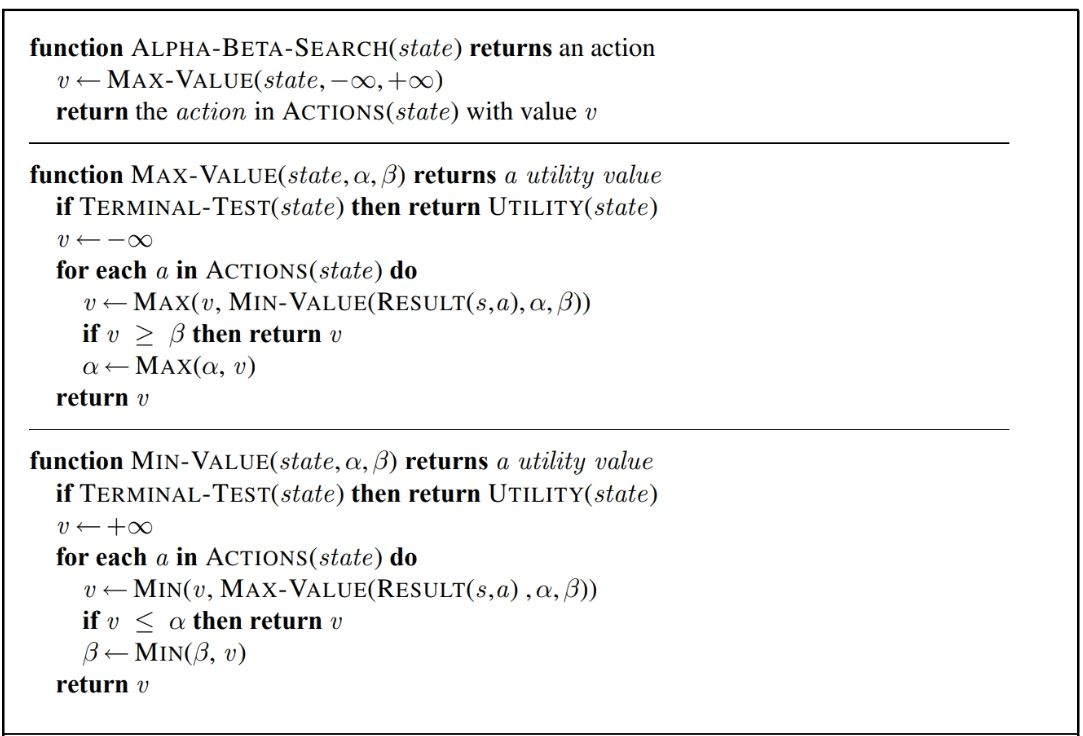
\includegraphics[width=\columnwidth]{AlphaBetaCode.JPG}
\caption{The Alpha-Beta pseudo code, from Russell and Norvig's AI textbook~\cite{russell2016artificial}.}
\label{fig:alpha-beta-code}
\end{figure}

% Heuristics
The size of the game tree is often too large to search, and many improvements and variants of the Minimax algorithm have been proposed. A common approach is to limit the depth of the search, and to estimate ``leaves'' that are not terminal states by a heuristic function. Using a heuristic function to evaluate non-terminal states is common when developing AI players. When using a heuristic, however, the value obtained when running the Minimax algorithm can be different from the minimax value of the game. 

% Alpha Beta
An orthogonal improvement that is the focus of this work is the famous Alpha-Beta pruning method. 
Figure~\ref{fig:alpha-beta-code} lists the pseudo-code of Alpha-Beta as given by the standard Russell and Norvig AI textbook (\citeyear{russell2016artificial}). 
%~\cite{KnuthAndFriend}.[[Roni: not clear who is the origin of alpha-beta]]
When using Alpha-Beta pruning, every searched node $n$ maintains two values $\alpha(n)$ and $\beta(n)$. 
Informally, the Alpha-Beta pruning rule says that if $\MM(n)$ is smaller than $\alpha(n)$ or larger than $\beta(n)$ then $n$ can be pruned, i.e., the minimax value of the game can be found without expanding $n$. In more details,  
$\alpha(n)$ is initialized to $\vmin$ for $\rootnode{}$ and to $\alpha(p(n))$ for all other nodes, and $\beta(n)$ is initialized to $\vmax$ for $\rootnode{}$ and to $\beta(p(n))$ for all other nodes. If a MAX node has a child that returns a value larger than $\alpha(n)$ then $\alpha(n)$ is updated to that value. Similarly, if $n$ is a MIN node and has a child that returns a value smaller than $\beta(n)$ then $\beta(n)$ is updated to that value. The Alpha-Beta pruning rules states that a state is pruned if $\alpha(n)\geq \beta(n)$.


Many improvements and variants of Alpha Beta have been proposed throughout the years, including searching with narrower ($\alpha, \beta$) window and changing it dynamically~\cite{pearl1980scout,reinefeld1983improvement}, using transposition tables, and using sophisticated child ordering. See
Schaeffer and Plaat (\citeyear{schaeffer1996new}) for a survey. 

%[[Abda: I don't understand the sentence staring with "These values". And what is $p(n)$?]][[Roni: Fixed and added def. of p(n) and C(n) earlier]]



% But, not good enough in many cases. 
%However, there is no known technique to obtain this best-case reduction (although there are heuristic methods that try to do so~\cite{AnyoneKnows}) and in the worst case Alpha-Beta pruning provides no speedup. In addition, there are still many games that are still too large to be solved, even with Alpha-Beta pruning. [[Abda: The first sentence is misleading: in practice, we are very very close to this best-case reduction using all sorts of optimizations. I think the right term is "effective branching factor" but I don't remember which one is the right paper to cite.]] [[Roni: if we have time tomorrow let's discuss this]]

\subsection{Games with Chance}
% The expectiminimax algorithm and a hint of Star 1
Game tree search algorithms such as Minimax and Alpha-Beta have well-known counterparts for games with chance.
The ExpectiMax algorithm~\cite{michie1966game} performs a depth-first search to find the minimax value of games with chance.
The *-Minimax~\cite{ballard1983minimax} family of algorithms adapt Alpha-Beta pruning to games with chance. The high-level idea of these pruning techniques is to consider the value of unexplored children of CHANCE nodes as any value between $\vmin$ and $\vmax$ and prune accordingly. 

In more details, *-Minimax algorithms maintain two values for every explored node $n$, $\pess(n)$ and $\opti(n)$, which maintain lower and upper bounds, respectively, on the minimax value of $n$. 
$\pess(n)$ is initialized to $\vmin$ and $\opti(n)$ to $\vmax$. 
MIN nodes update $\opti(n)$ so that $\opti(n)$ is the minimum over the $\opti$ values of all its explored children. Analogously, MAX nodes update $\pess(n)$. CHANCE nodes update $\opti(n)$ to be the expectation over the $\opti(n)$ value of its children, assuming $\vmax{}$ for every unexplored child, and update $\pess(n)$ to be the expectation over the $\pess(n)$ value of its children, assuming $\vmin{}$ for every unexplored child. 
The $\alpha$ and $\beta$ values of a node $n$ are then derived from $\opti(n)$ and $\pess(n)$. For more details see~\cite{hauk2004rediscovering}. 

% to the minimum over the $\pess$ value of the explored child nodechild no and get updated as children of $n$ are explored.  MAX nodes update $\opti(n)$  When a child node 
%[[Roni: Ideally, add here more explanations on how *-Minimax works without talking about pess and opti]]
%[[Abda: That would be a bit hard because the existing papers on *-minimax already use L and U to make it understandable.]][[Roni: I tried]]
%For completeness, we describe here one specific algorithm from the *-Minimax family called Star 1 [[Roni: Abdallah, if you have a sentence to write here on why we focus on Star 1, that'd be great]], and then present our general theory for bounded pruning in games of chance. 
%\subsection{Star 1}
%We Follow Lanctot et al.~\cite{lanctot2013} and describe Star 1 using  Alpha-beta pruning was introduced to games with chance in the Star-1 and Star-2 algorithms~\cite{TODO}. In this section we build on this prior work and extend Theorem~\ref{the:basic} to games with chance. 

 

%---------------------------------------------------------
%---------------------------------------------------------


\section{Finding a Bounded-Suboptimal Solution}

% Problem definition
The pruning done by Alpha-Beta and *-Minimax are \emph{safe}, in the sense that the minimax value the search ends up with is exactly the same as the minimax value obtained without the pruning. In the best case, one can obtain a square root reduction in the number of generated states for uniform game trees~\cite{knuth1975analysis,ballard1983minimax}. In the worst case, however, no pruning occurs. Even with these pruning techniques, computing the exact minimax value of many games is still not feasible. %[[Roni: Abdallah - do you have nice references to put here]]  

When this occurs in single-agent search, a common approach is to trade-off solution quality for runtime~\cite{pohl1970heuristic,thayer2011bounded,gilon2016dynamic}. 
In this work, we propose a method for doing this for game tree search, when searching for the minimax value. 
To define solution quality in this context, we say that an  \emph{optimal} solution to a game corresponds to finding its exact minimax value, and the \emph{suboptimality} of any other solution is its absolute difference from the minimax value. %[[suboptimality can also be ratio]] 
Thus, a \emph{bounded-suboptimal} game tree search algorithm is defined as a game tree search algorithm that accepts $\epsilon \geq 0$ as input and outputs a solution with suboptimality at most $\epsilon$. 
Naturally an effective bounded-suboptimal game tree search algorithm is also expected to provide stronger pruning for larger values of $\epsilon$.
To the best of our knowledge, there are no bounded-suboptimal game tree search algorithms in the literature. 

\subsection{Na\"{\i}ve Approach}
% A straightforward approach
Consider first only deterministic games, and the following straightforward approach to adapt Alpha-Beta to be a bounded suboptimal game tree search algorithm.
Instead of pruning a node $n$ only when $\beta(n) \leq \alpha(n)$ (see the 5th line the \texttt{Max-Value} and \texttt{Min-Value} functions in Figure~\ref{fig:alpha-beta-code}), prune $n$  when $\beta(n) \leq \alpha(n) +\epsilon$. 

While this simple Alpha-Beta adaption may prune larger parts of the game tree compared to regular Alpha-Beta, the resulting suboptimality, however, is not bounded by $\epsilon$.
To see this, consider the following example. 

\begin{figure}
	\centering
	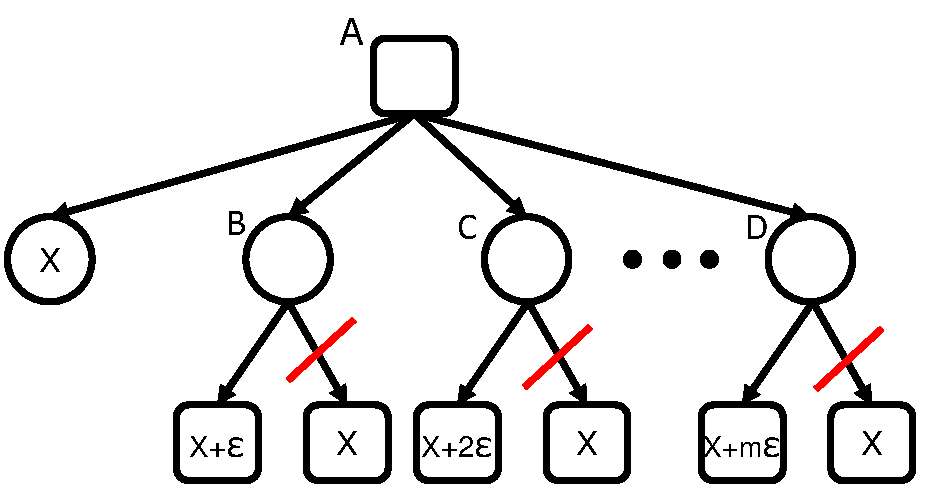
\includegraphics[width=0.85\columnwidth]{Figures/example_e.pdf}
	\caption{Example of adding $\epsilon$ to the standard alpha-beta}
	\label{fig:example-e}
\end{figure}

Considering we execute the standard alpha-beta algorithm with a pruning rule of $\beta(n) \leq \alpha(n)+\epsilon$ on the tree presented in Figure~\ref{fig:example-e} (squares represent MAX nodes and circles represent MIN nodes).
We explore first the root and then its leftmost child, update $\alpha(A)=X$, and transmit it to node $B$.
We explore the left child of node $B$ and update $\beta(B)=X+\epsilon$, then we prune its right child, return its value of $X+\epsilon$ up to $A$, update $\alpha(A)$ to $X+\epsilon$, and transmits it to node $C$. 
After we explored the left child of node $C$, we update $\beta(C)=X+2\epsilon$, prune its right child and return $X+2\epsilon$ to the root.
This procedure can go on and on until $X+m\epsilon$ (node $D$) for every possible positive value of $m$.
At the end of the algorithm execution, the value of the root is $X+m\epsilon$ despite the fact that the minimax value in this example is $X$ and that this gap is greater than the value of $\epsilon$.

%The root explores first its leftmost child, updates $\alpha=X$, and transmits it to node $B$.
%Node $B$ explores its left child and updates $\beta=X+\epsilon$, then it prunes its right child, and returns its value of $X+\epsilon$ up to $A$ which updates $\alpha$ to $X+\epsilon$ and transmits it to node $C$.
%After node $C$ explored its left child, it updates $\beta=X+2\epsilon$, prunes its right child and return $X+2\epsilon$ to the root.
%This procedure can go on and on until $X+m\epsilon$ (node $D$) for every possible positive value of $m$.
%At the end of the algorithm execution, the value of the root is $X+m\epsilon$ despite the fact that the minimax value in this example is $X$ and that this gap is greater than the value of $\epsilon$.

%[[Abda: we don't need to set $\epsilon = 1$. It suffices to have values $x+\epsilon$, $x+2\epsilon$, ..., $x+m\epsilon$. So the counter-example works with any positive value of epsilon.]] [[Roni: Agreed, TODO if time permits]] [[Dor: I changed it]]

Next, we present our pruning rule, which is guaranteed to preserves the desired suboptimality bound and is applicable to both deterministic games and games with chance. 

\subsection{Bounded-Suboptimal Pruning Rule}
%To present our pruning rule, we use the terminology of Cazenave and Saffidine~\cite{computerAndGames2011} for describing Alpha Beta pruning. 
Let $G$ be a game tree of some game, $A$ be a game tree search algorithm, and $A(G)$ be the subtree of $G$ that includes all the nodes generated by $A$ when run on $G$.
We assume that $A(G)$ is connected and has the same root as $G$. 
$C_A(n)$ denotes the children of $n$ that are in $A(G)$. Of course $C_A(n)\subseteq C(n)$.  
The nodes in $A(G)$ can be divided to three types: \emph{leaves}, \emph{partially expanded}, and \emph{fully expanded}.
A node is a \emph{leaf} in $A(G)$ if none of its children are in $A(G)$.
Note that a leaf in $A(G)$ may or may not be a terminal node (leaf) in $G$.  
A node in $A(G)$ is \emph{fully expanded} if all its children are in $A(G)$.
Every node in $A(G)$ that is not a leaf node and is not fully expanded is called a \emph{partially expanded} node. 
Partially expanded nodes correspond to nodes with pruned children.
In order to prune children of chance nodes, Lanctot et al. (\citeyear{lanctot2013monte}) used lower and upper bounds. Below, we use these bounds to achieve a bounded suboptimal minimax value.
Following Lanctot et al., we define $\pess$, $\opti$, $\alpha$, and $\beta$ for nodes in $A(G)$, as follows. 
Each of these four maps associates nodes in $A(G)$ to values in $[\vmin, \vmax]$. Roughly, $\pess(n)$ and $\opti(n)$ represent the tightest lower and upper bounds, respectively, on the minimax value of $n$  obtained by running $A$ on $G$, and if $\MM(n)$ is not in the range $[\alpha(n),\beta(n)]$ then it will not impact the minimax value of its parent. Formally, $\pess$, $\opti$, $\alpha$, and $\beta$ must satisfy the following conditions. 

%, and they satisfy the following conditions. 
%We will show that if these values satisfy some conditions, then they can be used as the basis of a pruning algorithm with bounded-suboptimality guarantees.
\noindent C1. For every non-leaf MAX node $n$:\\ 
 \indent (1) $\pess(n)=\max_{c\in C_A(n)} \pess(c)$\\
 \indent (2) $\opti(n)=\vmax$ if $n$ is partially expanded \\
 \indent (3) $\opti(n)=\max_{c\in C_A(n)} \opti(c)$ if $n$ is fully expanded.\\[2mm]
\noindent C2. For every non-leaf MIN node $n$:\\
\indent (1) $\opti(n)=\min_{c\in C_A(n)} \opti(c)$ \\
\indent (2) $\pess(n)=\vmin$ if $n$ is partially expanded \\
\indent (3) $\pess(n)=\min_{c\in C_A(n)} \pess(c)$ if $n$ is fully expanded\\[2mm]
\noindent C3. For every non-leaf CHANCE node $n$:\\ 
\indent (1) $\pess(n)= \sum\limits_{c\in C_A(n)} \pi(c) \pess(c) + (1-\sum\limits_{c\in C_A(n)} \pi(c)) \vmin{}$ \\
\indent (2) $\opti(n)= \sum\limits_{c\in C_A(n)} \pi(c) \opti(c) + (1-\sum\limits_{c\in C_A(n)} \pi(c)) \vmax{}$ \\[2mm]
\noindent C4. For the root $n_1$, $\alpha(\rootnode)=\pess(\rootnode)$ and $\beta(\rootnode)=\opti(\rootnode)$\\[2mm]
\noindent C5. For every MAX or MIN node $n$ that is not the root and every child node $c\in C_A(n)$:\\
\indent (1) $\alpha(c)=\max(\alpha(n),\pess(c))$\\
\indent (2) $\beta(c)=\min(\beta(n),\opti(c))$ \\[2mm]
\noindent C6. For every CHANCE node $n$  that is not the root and every child node $c \in C_A(n)$:\\
\indent (1) $\alpha(c) = \max(\pess(c), \frac{\alpha(n)-\opti(n)}{\pi(c)}+\opti(c))$ \\
\indent (2) $\beta(c) = \min(\opti(c), \frac{\beta(n)-\pess(n)}{\pi(c)}+\pess(c))$\\


%In the rest of this section, we assume given $\pess$, $\opti$, $\alpha$, and $\beta$, four arbitrary functions satisfying the above conditions.[[ I don't see why we need this. We defined these functions as functions that satisfy these conditions ]]
First, we establish that $\pess$ and $\opti$ constitute admissible bounds for all nodes of the tree.

\begin{lemma}
  If for every leaf node $n$ it holds that $\MM(n)\in [\pess(n), \opti(n)]$, then it also holds for all other nodes in $A(G)$.
\label{lem:opti-pess}
\end{lemma}
\begin{proof}
We prove Lemma~\ref{lem:opti-pess} by induction on the height of the nodes. For the base case, nodes of height 0 are leaves, and the statement is an assumption of the lemma.
%For the base case, nodes of height 0 are leaves, the statement holds from condition C1.

For the induction step, let us assume that for any node $n$ of height $\leq H$, we have $\pess(n)\!\leq\! \MM(n)\!\leq\! \opti(n)$ and let us prove that this also holds for nodes of height $H+1$.
For a node $n$ of height $H+1$, any child $c \in C_A(n)$ has height $\leq H$, so in particular $\pess(c)\!\leq\!\MM(c)\!\leq\!\opti(c)$ (induction hypothesis).

\paragraph{Case \#1: $n$ is a MAX node.}
$C_A(n) \subseteq C(n)$, so we have
\begin{align}
  \pess(n) = \!\!\!\!\max_{c\in C_A(n)} \!\!\!\!\pess(c) \leq \!\!\!\!\max_{c\in C_A(n)} \!\!\!\!\MM(c) \leq \!\!\!\!\max_{c\in C(n)} \!\!\!\! \MM(c) \! = \!\!\MM(n)
\end{align}
If $n$ is fully expanded, then $C_A(n)=C(n)$ and so
\begin{align}
  \MM(n) \!= \!\!\!\max_{c \in C(n)} \!\!\!\!\MM(c) \!= \!\!\!\!\max_{c \in C_A(n)} \!\!\!\!\MM(c) \leq \!\!\!\!\max_{c \in C_A(n)} \!\!\!\!\opti(c) \!= \!\!\opti(n)
\end{align}
Else, $n$ is partially expanded and so $\MM(n) \leq \vmax = \opti(c)$.
Thus, in all cases it holds that $\pess(n) \leq \MM(n) \leq \opti(n)$.

%[[TODO: RE-CONSIDER ORDERING OF INEQUALITIES]]

\paragraph{Case \#2: $n$ is a MIN node.}
$C_A(n) \subseteq C(n)$, so we have
\begin{align}
  \MM(n) \!= \!\!\!\!\min_{c\in C(n)} \!\!\!\!\MM(c) \leq \!\!\!\!\min_{c\in C(n)} \!\!\!\!\opti(c) \leq \!\!\!\!\min_{c \in C_A(n)} \!\!\!\! \opti(c) \! = \! \opti(n)
\end{align}
If $n$ is fully expanded, then $C_A(n)=C(n)$ and so
\begin{align}
  \pess(n) \! = \!\!\!\!\min_{c \in C_A(n)} \!\!\!\!\pess(c) \leq \!\!\!\!\min_{c \in C_A(n)} \!\!\!\!\MM(c) = \!\!\!\!\min_{c \in C(n)} \!\!\!\!\MM(c) \!=\! \MM(n)
\end{align}
Else, $n$ is partially expanded and so $\pess(c) = \vmin\leq \MM(n)$. 
Thus, in all cases it holds that $\pess(n) \leq \MM(n) \leq \opti(n)$.

\paragraph{Case \#3: $n$ is a CHANCE node.}
For every child $c$ it holds that $\vmin\leq \MM(c)$. 
Also, $1-\sum_{c\in C_A(n)} \pi(c) = \sum_{c\in C(n) \setminus C_A(n)} \pi(c)$. Following C3(1) we have
%Since $\vmin\leq \MM(c) \leq \vmax$ we have
\begin{align}
 \pess(n) = & \!\sum_{c\in C_A(n)\!\!\!\!\!} \!\!\!\pi(c) \pess(c)+ (1-\!\!\!\sum_{c\in C_A(n)\!\!\!\!\!}\!\! \pi(c)) \vmin \\
 \pess(n) \leq & \!\sum_{c\in C_A(n)\!\!\!\!\!} \!\!\!\pi(c) \MM(c)+ \!\!\!\!\sum_{c\in C(n) \setminus C_A(n)\!\!\!\!\!\!\!\!\!\!\!\!}\!\!\!\!\!\pi(c) \MM(c) = V(n)
\end{align}
Similarly
\begin{align}
 \MM(n) = \!\sum_{c\in C_A(n)\!\!\!\!\!} \!\!\!\pi(c) \MM(c)+ \!\!\!\!\sum_{c\in C(n) \setminus C_A(n)\!\!\!\!\!\!\!\!\!\!\!\!}\!\!\!\!\!\pi(c) \MM(c) \leq \opti(n)
\end{align}
Thus, $\pess(n) \leq \MM(n) \leq \opti(n)$ as required.
\end{proof}

Second, we make the following straightforward observation, based on conditions C4--C6.

\begin{lemma}
For any node $n$, $\pess(n) \!\leq\! \alpha(n)$ and $\beta(n) \leq \opti(n)$.
\label{lem:alpha-beta-between-l-u}
\end{lemma}

Third, we prove that $\epsilon$ bounds coming from leaves and pruned nodes propagate through the tree without increasing.

\begin{lemma}
If $\beta(n)\leq \alpha(n)+\epsilon$ holds for all leaf nodes and all partially expanded nodes, then it also holds for all other nodes in $A(G)$. 
\label{lem:bounded-beta}
\end{lemma}
\begin{proof}
We prove Lemma~\ref{lem:bounded-beta} by induction on the height of the nodes.
For the base case, nodes of height 0 are leaves, and the statement is an assumption of the lemma.

For the induction step, let us assume that for any node $n$ of height $\leq H$, we have $\beta(n)\leq \alpha(n)+\epsilon$ and let us prove that this also holds for nodes of height $H+1$.
For a node $n$ of height $H+1$, any child $c \in C_A(n)$ has height $\leq H$, so in particular $\beta(c)\leq \alpha(c)+\epsilon$ (the induction hypothesis).

\paragraph{Case \#1: $n$ is a MAX node.}
For every child $c$, applying condition C5 to the induction hypothesis gives the inequality
$\min(\beta(n), \opti(c)) \leq \max(\alpha(n), \pess(c))+\epsilon$.
Therefore 
\begin{align}
\!\!\max_{c \in C(n)} \!\!\min(\beta(n), \opti(c)) \leq & \!\!\max_{c \in C(n)} \!\!\max(\alpha(n), \pess(c))+\epsilon\\
\!\!\min(\beta(n), \!\!\max_{c \in C(n)}\!\!\opti(c)) \leq & \max(\alpha(n), \!\!\max_{c \in C(n)}\!\!\pess(c))+\epsilon\\
\!\!\min(\beta(n), \opti(n)) \leq & \max(\alpha(n), \pess(n))+\epsilon
\end{align}
From Lemma~\ref{lem:alpha-beta-between-l-u} conclude that $\beta(n) \leq \alpha(n) + \epsilon$.

\paragraph{Case \#2: $n$ is a MIN node.}
Similarly to Case \#1 we have 
\begin{align}
\!\!\min_{c \in C(n)} \!\!\min(\beta(n), \opti(c)) \leq & \!\!\min_{c \in C(n)} \!\!\max(\alpha(n), \pess(c))+\epsilon\\
\!\!\min(\beta(n), \!\!\min_{c \in C(n)}\!\!\opti(c)) \leq & \max(\alpha(n), \!\!\min_{c \in C(n)}\!\!\pess(c))+\epsilon\\
\!\!\min(\beta(n), \opti(n)) \leq & \max(\alpha(n), \pess(n))+\epsilon
\end{align}
Leading to the desired result, $\beta(n) \leq \alpha(n) + \epsilon$.

\paragraph{Case \#3: $n$ is a CHANCE node.} 
For every child node $c$, using condition C6 gives the two equalities 
$\alpha(c)=\max(\pess(c), \frac{\alpha(n)-\opti(n)}{\pi(c)}+\opti(c))$
and $\beta(c)=\min(\opti(c), \frac{\beta(n)-\pess(n)}{\pi(c)}+\pess(c))$.
Consider each of the four possible assignments for $\alpha(c)$ and $\beta(c)$. 


\noindent \textbf{Case \#3.1: there is a child $c\in C_A(n)$ such that 
\[\alpha(c)=\frac{\alpha(n)-\opti(n)}{\pi(c)}+\opti(c) 
\text{ and } \beta(c)=\opti(c)\]}
\noindent The induction hypothesis gives
\begin{align}
\opti(c) \leq & \frac{\alpha(n)-\opti(n)}{\pi(c)}+\opti(c)+\epsilon \\
\opti(n) \leq & \alpha(n) + \pi(c)\epsilon
\end{align}
Since $\beta(n)\!\leq\!\!\opti(n)$ and $0\!\leq\!\pi(c)\!\leq\!1$, we get $\beta(n)\!\leq\!\alpha(n) + \epsilon$.

\textbf{Case \#3.2: there is a child $c\in C_A(n)$ such that
\[ \alpha(c)=\pess(c) \text{ and } \beta(c)=\frac{\beta(n)-\pess(n)}{\pi(c)}+\pess(c) \]}
\noindent The induction hypothesis gives
\begin{align}
\frac{\beta(n)-\pess(n)}{\pi(c)}+\pess(c) \leq & \pess(c)+\epsilon \\
\beta(n) \leq & \pess(n) + \pi(c) \epsilon
\end{align}
As $\pess(n) \leq \alpha(n)$ and $\pi(c)$$\in$$[0,1]$, we get $\beta(n) \leq \alpha(n) + \epsilon$.


\textbf{Case \#3.3: there is a child $c\in C_A(n)$ such that 
\[\alpha(c)=\frac{\alpha(n)-\opti(n)}{\pi(c)}+\opti(c) \text{ and } \beta(c)=\frac{\beta(n)-\pess(n)}{\pi(c)}+\pess(c)\]}
%$\alpha(c)=\frac{\alpha(n)-\opti(n)}{\pi(c)}+\opti(c)$ and $\beta(c)=\frac{\beta(n)-\pess(n)}{\pi(c)}+\pess(c)$.}
 
\noindent The induction hypothesis gives
\begin{align}
\frac{\beta(n)-\pess(n)}{\pi(c)}+\pess(c) &\leq \frac{\alpha(n)-\opti(n)}{\pi(c)}+\opti(c) + \epsilon\label{eq:3.3-a}
%\beta(n)-\pess(n)+\pi(c)\cdot \pess(c) &\leq  \alpha(n)-\opti(n)+\pi(c)\cdot\opti(c) + \pi(c)\cdot \epsilon\label{eq:3.3-a2}
\end{align}
Since $c\in C_A(n)$, then we have
\begin{align}
\pi(c)(\opti(c)-\pess(c)) \leq & \!\!\sum_{c'\in C_A(n)\!\!\!\!\!\!\!\!\!} \!\pi(c')(\opti(c')-\pess(c'))\\
\pi(c)(\opti(c)-\pess(c)) \leq & \opti(n)-\pess(n)\\
\pess(n) - \pi(c)\pess(c) \leq & \opti(n)-\pi(c)\opti(c) \label{eq:3.3-b}
\end{align}
Adding $\pi(c) \cdot$ Eq.~\eqref{eq:3.3-a} to Eq.~\eqref{eq:3.3-b} gives $\beta(n) \leq \alpha(n)+\pi(c)\epsilon$.

\textbf{Case \#3.4: for each child $c\in C_A(n)$ it holds that
\[ \alpha(c)=\pess(c) \text{ and } \beta(c)=\opti(c)\]}

%By definition of $n$, 
\noindent Since $\beta(c)\leq \alpha(c)+\epsilon$, we have that
\begin{align}
\sum_{c\in C_A(n)} \!\!\pi(c) \beta(c) \leq & \sum_{c\in C_A(n)} \pi(c)(\alpha(c) + \epsilon)\\
\sum_{c\in C_A(n)} \!\!\!\pi(c)\opti(c) \leq & \!\!\sum_{c\in C_A(n)} \!\!\!\!\pi(c)\pess(c) + \!\!\!\sum_{c\in C_A(n)} \!\!\!\!\pi(c)\epsilon \label{eq:opti-pess-eps}
\end{align}
Since $n$ is fully expanded, $\sum_{c\in C_A(n)} \pi(c) = 1$ and C3 gives
\begin{align}
\opti(n) \leq & \pess(n) + \epsilon \label{eq:opti-pess-eps}
\end{align}
from Lemma~\ref{lem:alpha-beta-between-l-u} conclude that $\beta(n) \leq \alpha(n) + \epsilon$.
\end{proof}


We are now fully equipped to prove the main theoretical contribution of this paper.

\begin{theorem}
For a game tree $G$, a game tree search algorithm $A$, 
and any $\epsilon\geq 0$, if all the following conditions hold
\begin{enumerate}
\item for every leaf node $n$
\[ \pess(n) \leq \MM(n) \leq \opti(n) \text{ and } \opti(n)-\pess(n)\leq \epsilon \]
\item for every partially expanded node $n$, 
$\beta(n) \leq \alpha(n)+\epsilon$
\end{enumerate}
then 
\[\MM(\rootnode)\in [\pess(\rootnode),\pess(\rootnode)+\epsilon]\]
\label{the:basic}
\end{theorem}
\begin{proof}
The first condition lets us apply Lemma~\ref{lem:opti-pess} and obtain for the root $\pess(n_1) \leq \MM(n_1) \leq \opti(n_1)$, and to apply Lemma~\ref{lem:alpha-beta-between-l-u} to obtain $\beta(n) \leq \alpha(n) + \epsilon$ for every leaf node $n$. 
Together with the second condition we can apply Lemma~\ref{lem:bounded-beta} for all nodes in $A(G)$.
In particular, we obtain for the root $\beta(n_1) \leq \alpha(n_1) + \epsilon$.
From condition C4, we conclude that $\opti(\rootnode)\leq \pess(\rootnode)+\epsilon$.
Therefore, $\pess(\rootnode) \leq \MM(\rootnode) \leq \pess(\rootnode) + \epsilon$ as intended.
\end{proof}
Note that in the above proof we prove that $\opti(\rootnode)\leq \pess(\rootnode)+\epsilon$. Therefore, if the conditions in Theorem~\ref{the:basic} hold, then it is also true that $\MM(\rootnode)\in [\opti(\rootnode)-\epsilon,\opti(\rootnode)]$. % This is here to address a concern by the reviewer


%\subsubsection{Redistributing $\epsilon$}
%Line~\ref{line:recursive} in Algorithm~\ref{alg:weightedAlphaBeta} is the recursive call for computing $\opti$ and $\pess$ of the child of the current node.  A deeper look on the proof of Theorem~\ref{the:chance} reveals that it is possible to provide more flexibility in how $\epsilon$ is distributed between the children of a chance node. Instead of passing $\epsilon$ to each child node, it is possible to provide different values of $\epsilon$ to different children of $n$.  Let $\epsilon(n)$ be the $\epsilon$ passed to a node $n$. The following condition is sufficient to maintain the  guarantee provided by Theorem~\ref{the:chance}  

%Instead of running each child of a chance node with the same $\epsilon$, one can use different values of $\epsilon$ for the there is a recursive call for 
%\begin{theorem} 	\label{theorem_error_bound} 	If for every chance node $n$ it holds that 	\[ \sum_{c\in C(n)} 			\epsilon(n) \leq \epsilon(n) \] 	and all the conditions specified in Theorem~\ref{the:chance} hold then  	 \MM(\rootnode)\in     [\pess(\rootnode),\pess(\rootnode)+\epsilon]$ \end{theorem} \begin{proof} 	TODO \end{proof}

%---------------------------------------------------------
%---------------------------------------------------------



%---------------------------------------------------------


\section{The Bounded Alpha-Beta (BAB) Algorithm} 
%Describing the pseudo code + improvement
 \refstepcounter{bab}
 \label{sec:bab}

\begin{algorithm}[t]
\DontPrintSemicolon
%\KwIn{$(n, p)$ - a game tree node and its parent}
\KwIn{$n$ - a game tree node}
%\KwIn{$(\alpha_p, \beta_p)$ - the $\alpha$ and $\beta$ values of the parent node}
\KwIn{$\epsilon$ - an error margin}

\If{$n$ is a terminal node}{
  \nllabel{line:term-start}
  %$\alpha = \max(\alpha_p, \eval(n))$; $\beta = \min(\beta_p, \eval(n))$\;
  \Return $( \MM(n), \MM(n) )$\;
  \nllabel{line:term-end}
}

$\pess(n)\gets \vmin$;
$\opti(n)\gets \vmax$\; \nllabel{line:init-start}
  \lIf{$n$ is a MAX node}{
  	$\besto \gets \vmin$
  }\lElseIf{$n$ is a MIN node}{
    $\bestp\gets \vmax$
  }
  
  \lIf{$n$ is $\rootnode$ \nllabel{line:alpha-update-start}}{
     $\alpha(n)=\vmin$; $\beta(n)=\vmax$
  }
  \lElseIf{$p(n)$ is a MAX node or a MIN node \nllabel{line:alpha-update-start}}{
     $\alpha(n)=\alpha(p(n))$; $\beta(n)=\beta(p(n))$
  }
  \Else{
    $\alpha(n)\gets \max(\vmin, \frac{\alpha(p(n))-\opti(p(n))}{\pi(n)} + \opti(n))$\;
    $\beta(n)\gets \min(\vmax, \frac{\beta(p(n))-\pess(p(n))}{\pi(n)} + \pess(n))$\;
    \nllabel{line:init-end}
  }
  
\ForEach{child $c$ of $n$}{
  \nllabel{line:loop-start}
  %$\zeta\gets$ ComputeChildBound($\epsilon$, $\opti(n)$,$\pess(n)$,$\pi(c)$)\;
  $\big(\pess(c),\opti(c)\big)\gets$ BoundedAB($c$, $\epsilon$) \nllabel{line:recursive}\;

  \If{$n$ is a MAX node}{
    \nllabel{line:lu-update-start}
    $\besto\gets \max(\besto,\opti(c))$\;
    $\pess(n)\gets \max(\pess(n),\pess(c))$\;
%    $\opti(n)\gets \max(\opti(n),\opti(c))$\; Always vmax
  }
  \ElseIf{$n$ is a MIN node}{
    $\bestp\gets \min(\bestp,\pess(c))$\;
%    $\pess(n)\gets \min(\pess(n),\pess(c))$\;  Always vmin
	$\opti(n)\gets \min(\opti(n),\opti(c))$\;
    \nllabel{line:lu-update-end-det}
  }\Else{
    $\pess(n)\gets \pess(n)+\pi(c)(\pess(c)-\vmin)$\; \nllabel{line:lu-update-chance-start}
%    $\opti(n)\gets \opti(n)+\pi(\opti(c)-\vmax)$\;
	$\opti(n)\gets \opti(n)-\pi(c)(\vmax-\opti(c))$
    \nllabel{line:lu-update-end}    
    \;
  } 

  $\alpha(n)\gets \max(\pess(n), \alpha(n))$\;
  $\beta(n)\gets \min(\opti(n), \beta(n))$\;
      
  \lIf{$\beta(n)\leq \alpha(n)+\epsilon$ and $c$ is not the last child of $n$}{
    \Return $(\pess(n),\opti(n))$
    \nllabel{line:break-loop}
  }  
}
\lIf{$n$ is a MAX node}{
  \nllabel{line:update-best-start}
  $\opti(n)\gets \besto$
}\lElseIf{$n$ is a MIN node}{
  $\pess(n)\gets \bestp$
  \nllabel{line:update-best-end}
}

\Return $(\pess(n),\opti(n))$\;

\caption{BoundedAB}
\label{alg:weightedAlphaBeta}
\end{algorithm}
Next, we described Bounded Alpha-Beta (BAB), which is a bounded-suboptimal game tree search algorithm 
that is based on the classical Alpha-Beta algorithm, *-Minimax algorithm, and our bounded-suboptimal pruning rule (Theorem~\ref{the:basic}). 
BAB performs a depth-first search on the game tree, maintains in each node its $\opti$ and $\pess$ values, computes its $\alpha$ and $\beta$ values based on the $\opti$ and $\pess$ values of its generated children, and prunes states whenever $\beta \leq \alpha+\epsilon$. Note that $\epsilon=0$ correspond to the standard alpha-beta algorithm.

%[[Roni: some uncleanliness in what we do in terminal nodes. Do we have a heuristic there or is it our utility function ($u(n)$)]]

Algorithm \ref{alg:weightedAlphaBeta} lists the pseudo code of BAB.
Lines \ref{line:term-start}--\ref{line:term-end} describe the case where $n$ is a leaf node and hence it returns $\MM(n)$. %\footnote{If the $\MM(n)$ is not available, a pair of heuristic functions can be used such that $\MM(n)$ is } 
%Later in the pseudo-code, in line \ref{line:recursive}, this value is assigned to its $\opti$ and $\pess$ parameters and therefore it holds condition $C1$ described in Theorem \ref{the:basic}.
Lines \ref{line:init-start}--\ref{line:init-end} initialize the $\pess$, $\opti$, $\alpha$, and $\beta$ values. In addition, we 
initialize $\bestp$ and $\besto$ to $\vmin{}$ for MIN nodes and $\vmax{}$ for MAX nodes, respectively.
These values keep track of the highest $\pess{}$ and the lowest $\opti{}$ in the generated children, are used later to update $\pess(n)$ and $\opti(n)$ (see lines~\ref{line:update-best-start}-\ref{line:update-best-end}). 
%[[Roni: nothappy with the besto bestp text ]]
Lines~\ref{line:alpha-update-start}-\ref{line:init-end} update $\alpha$ and $\beta$ according to the type of $n$. 
%Lines \ref{line:chance-init-start}--\ref{line:init-end} will be used later in the paper, in a non-deterministic games. 
Line \ref{line:loop-start} starts a transition over each child of the current node, and recursive call to BAB on that node is 
in line \ref{line:recursive}. Lines \ref{line:lu-update-start}--\ref{line:lu-update-end} updates 
the values of the relevant variables, and the actual pruning is done in line~\ref{line:break-loop}. 
Note that the computation of $\pess(n)$ and $\opti(n)$ for CHANCE nodes is done incrementally (lines~\ref{line:lu-update-chance-start}-\ref{line:lu-update-end}) by adding the new $\pess(c)$ and $\opti(c)$ values and subtracting the initial $\vmin$ and $\vmax$ values.


\subsubsection{Choosing a Bounded-Suboptimal Action}
BAB (Algorithm~\ref{alg:weightedAlphaBeta}) returns a range $[\pess(\rootnode), \opti(\rootnode)]$ for a given game tree and $\epsilon$. As proven in Theorem~\ref{the:basic}, the minimax value is in that range, and the size of the range is at most $\epsilon$. Thus, any value chosen in that range can serve as a bounded-suboptimal solution for the given $\epsilon$. 

To obtain a concrete policy from the output of BAB the MAX player needs to choose the action that leads to the highest $\pess$ values. This policy is guaranteed (on expectation) to provide at least a bounded-suboptimal minimax value, for any action the MIN player may choose. By contrast, choosing the action that leads to the highest $\opti$ values may end up with a strategy whose expected value is smaller than the minimax value by more than $\epsilon$. %Similarly, the MIN player can choose the action that leads to the lowest $\opti$ values in order to guarantee a bounded-suboptimal minimax value. [[Roni: I don't see the value in this, and it is confusing - the reader may be tempetd to thing we assume that the MIN player MUST do this. ]]



%---------------------------------------------------------

\subsubsection{Pruning Analysis}


Consider the amount of pruning that can be obtained when using BAB. Like Alpha-Beta and *-Minimax, in the worst case we still may need to generate all nodes in the game tree before halting, as long as $\epsilon<\vmax-\vmin$. 
Such a worst case occurs, for example, when the children of MAX nodes all lead to $\vmin$ except one node
and the children of MIN nodes all lead to $\vmax$ except one node, and this individual node is always generated last. 

In the best case, however, significant pruning can be achieved.
We conjecture that the best case cannot be better than that of Alpha Beta, except for the case where $\epsilon=\vmax-\vmin$, in which only a single branch in the game tree will be expanded, but the resulting value is not helpful. 
% This is in contrast to Alpha-Beta's worst case, which is exponential in half the depth of the game tree.


In general, we expect that  BAB with  $\epsilon_2$ will prune more nodes than BAB with $\epsilon_1$, if $\epsilon_2 > \epsilon_1$.
We verify experimentally later in this paper that this occurs in practice in most cases. 
However, in some special cases, BAB with $\epsilon_2$ actually prunes fewer nodes than BAB with $\epsilon_1$. 


\begin{figure}
	\centering
    \hfill\subfloat[$\epsilon=2$]{
  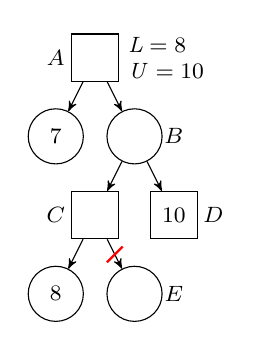
\begin{tikzpicture}[yscale=-1]
    \node[maxnode] (s0)  at (1.5, 0) {};
%    \node[maxnode] (s0)  at (1.5, 0) {$\pess=8$\\$\opti=10$};
    \node[minnode] (s1) at (1.0, 1) {$7$};
    \node[minnode] (s2) at (2.0, 1) {};
    \node[maxnode] (s3) at (1.5, 2) {};
    \node[maxnode] (s4) at (2.5, 2) {$10$};
    \node[minnode] (s5) at (1.0, 3) {$8$};
    \node[minnode] (s6) at (2.0, 3) {};
    \node[infobox] (i0) at ($(s0) + (-0.5, 0)$) {$A$};
    \node[infobox] (i2) at ($(s2) + (0.5, 0)$) {$B$};
    \node[infobox] (i3) at ($(s3) + (-0.5, 0)$) {$C$};
    \node[infobox] (i4) at ($(s4) + (0.5, 0)$) {$D$};
    \node[infobox] (i6) at ($(s6) + (0.5, 0)$) {$E$};
    \node[infobox] (i0ul) at ($(s0) + (+0.9, 0)$) {$\pess=8$\\$\opti=10$};
    
    \draw[->] (s0)  -- (s1);
    \draw[->] (s0)  -- (s2);
    \draw[->] (s2)  -- (s3);
    \draw[->] (s2)  -- (s4);
    \draw[->] (s3)  -- (s5);
    \draw[->] (s3)  -- (s6);
    \draw[thick,draw=red] ($(s3) + (0.35, 0.4)$) -- ($(s3) + (0.15, 0.6)$);
  \end{tikzpicture}}\hfill
  \subfloat[$\epsilon=1$]{
  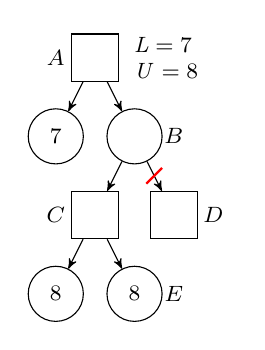
\begin{tikzpicture}[yscale=-1]
    \node[maxnode] (s0)  at (1.5, 0) {};
%    \node[maxnode] (s0)  at (1.5, 0) {$\pess=8$\\$\opti=10$};
    \node[minnode] (s1) at (1.0, 1) {$7$};
    \node[minnode] (s2) at (2.0, 1) {};
    \node[maxnode] (s3) at (1.5, 2) {};
    \node[maxnode] (s4) at (2.5, 2) {};
    \node[minnode] (s5) at (1.0, 3) {$8$};
    \node[minnode] (s6) at (2.0, 3) {$8$};
    \node[infobox] (i0) at ($(s0) + (-0.5, 0)$) {$A$};
    \node[infobox] (i2) at ($(s2) + (0.5, 0)$) {$B$};
    \node[infobox] (i3) at ($(s3) + (-0.5, 0)$) {$C$};
    \node[infobox] (i4) at ($(s4) + (0.5, 0)$) {$D$};
    \node[infobox] (i6) at ($(s6) + (0.5, 0)$) {$E$};
    \node[infobox] (i0ul) at ($(s0) + (+0.9, 0)$) {$\pess=7$\\$\opti=8$};
    
    \draw[->] (s0)  -- (s1);
    \draw[->] (s0)  -- (s2);
    \draw[->] (s2)  -- (s3);
    \draw[->] (s2)  -- (s4);
    \draw[->] (s3)  -- (s5);
    \draw[->] (s3)  -- (s6);
    \draw[thick,draw=red] ($(s2) + (0.35, 0.4)$) -- ($(s2) + (0.15, 0.6)$);
  \end{tikzpicture}}\hfill~
%	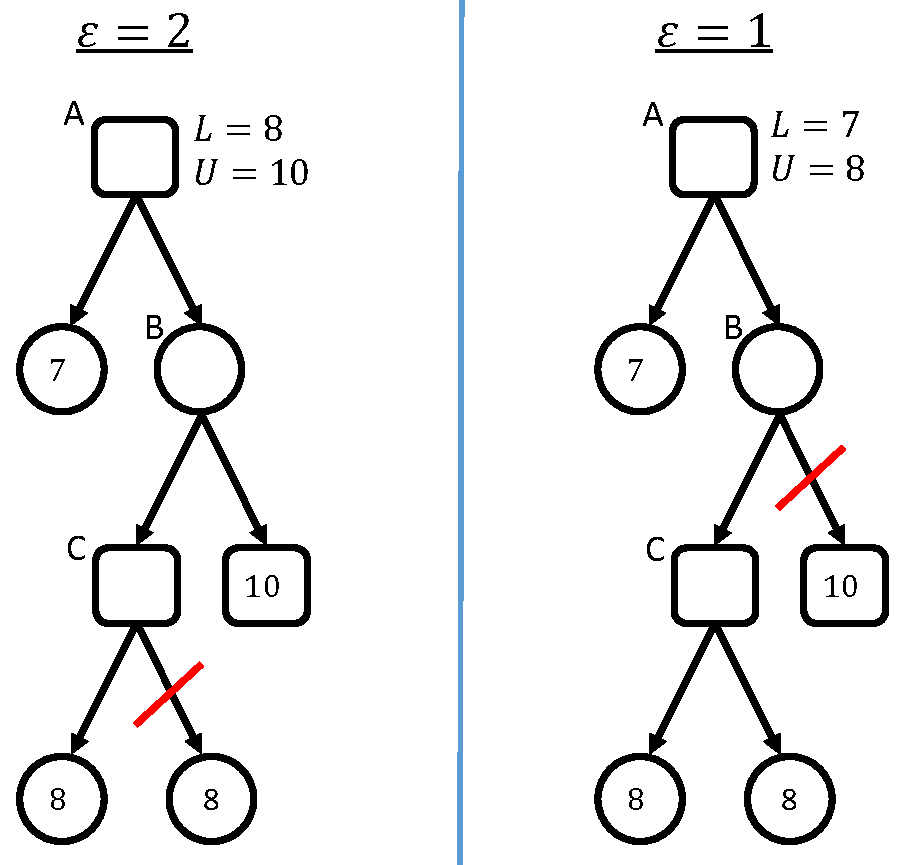
\includegraphics[width=0.6\columnwidth]{Figures/cropped_example_different_e.pdf}
	\caption{Example of BAB pruning with different suboptimality values. Depending on the relative size of the subtrees rooted in $D$ and $E$, $\epsilon = 2$ may lead to more or less pruning than $\epsilon = 1$.}
	\label{fig:bab-prune}
\end{figure}

Figure \ref{fig:bab-prune} demonstrate this phenomenon. The right tree represent an example of BAB with $\epsilon = 1$ and the left one represent BAB with $\epsilon = 2$. In both cases $\vmin = 0$ and $\vmax = 10$. In both cases, after we explored the left child of node $A$, we update $\alpha = 7$ and $\beta = 10$. These values transmitted down to $B$ and from there to $C$. After we explored the left child of node $C$, $\alpha = 8$ and $\beta = 10$. In this point, the left tree prune the right branch and the values that return to $B$ are $(8,10)$, we update the $\beta$ value of node $B$ to $10$ and explore the right child. In the right tree, the right child of $C$ does not get pruned and the values that return to $B$ are $(8,8)$, we update the $\beta$ value of node $B$ to $8$ and the right child get pruned.
%node $A$ explored the left child its $\alpha = 7$ and $\beta = 10$. These values transmitted down to $B$ and from there to $C$. After $C$ explored the left child $\alpha = 8$ and $\beta = 10$. In this point, the left tree prune the right branch and the values that return to $B$ are $(8,10)$, node $B$ update $\beta$ value to $10$ and explore the right child. In the right tree, the right child of $C$ does not get pruned and the values that return to $B$ are $(8,8)$, $B$ update $\beta$ value to $8$ and the right child get pruned. 
Although these two examples explored the same amount of nodes, the branch of the right child of $B$ and the branch of the right child of $C$ could contain large sub-trees and hence a greater $\epsilon$ value might explore less, more or equal amount of nodes. 


%---------------------------------------------------------
%---------------------------------------------------------





\section{Experimental Results}

% Evaluation metrics
In this section, we evaluate BAB experimentally. 
The main purpose of this evaluation is to measure the advantage and disadvantages of using our bounded pruning compared to the standard pruning provided by Alpha-Beta pruning and *-Minimax algorithm. We focus on two metrics: \emph{Expanded Ratio ($\er$)} and \emph{Actual Minimax Bound ($\amb$)}.
$\er$ is the amount of expansions divided by the amount of expansions done by the corresponding safe pruning method (i.e., BAB with $\epsilon=0$). Smaller $\er$ corresponds to a faster search. 
$\amb$ is the absolute difference between the $\opti$ value and the $\pess$ value of the root. Smaller $\amb$ means higher solution quality, as the bound around the true minimax value is smaller.
Theorem~\ref{the:basic} ensures that $\amb$ is no more than $\epsilon$.

%For instance, if BAB with $\epsilon=5$ expanded $9$ nodes and Alpha Beta expanded 10 nodes, we would obtain $\er = 0.9$ for BAB with $\epsilon=5$ on this instance.
%In addition, we measured the actual minimax bound, denoted AMB, returned by the evaluated algorithm, i.e., the gap between the $\opti$ value and the $\pess$ value of the root. %For example, $\amb(4)=3$ indicates that for $\epsilon=4$ the $\opti-\pess$ value is equal to $3$. [[Roni: example seems redundant to me]]
%Note that the AMB of BAB is at most $\epsilon$, as proven by Theorems~\ref{the:basic} and~\ref{the:chance}, 



\subsection{Domains}
% Domains
We evaluated BAB on two domains---random trees (RT) and a cops and robbers (C\&R) scenario~\cite{moldenhauer2009evaluating}. The games in the RT domain are randomly generated trees with a fixed depth and branching factor. We experimented with 
fixed depths of $3$, $5$, $7$, and $9$, and fixed branching factors of $2$, $3$, $4$, and $5$. 
The utility of leaves of these trees were drawn uniformly in the range $[0, 100]$. 

In the C\&R games, we randomly allocated $n$ cops and one robber on a 4-connected 6$\times$6 grid. The cops and the robber can move in their turn to one of their neighboring grid cells or stay in their current location. The robber is a MAX player and the cops are the MIN player, and all cops move simultaneously. The game ends when one of the cops reaches the robber. The score is the time until the robber is caught. 
In our experiments, we limited the depth of the C\&R games, and used the average Manhattan distance between all cops to the robber as a heuristic for the leaf nodes. We experimented with fixed depth of $1$, $3$, $5$, and $7$.
%We limited the depth of this game, a In this game we used the same heuristic for both player, which is the time elapsed + the average manhattan distance of all cops. 
%In our experiments we set the fix depth and branching factor were parameters of the tree were given a utility randomly  The random trees 

 %$\vmin=0$, $\vmax=10,000$

For the experiments on games with chance, we modified both domains to include a stochastic element, as follows. In the stochastic RT games, after a player chooses a move the move occurs with probability $p$, and every other move occurs with probability $\frac{1-p}{b-1}$, where $p$ is a parameter that we set to $0.8$ and $b$ is the branching factor. Here also, the utility of leaves of these trees were drawn uniformly in the range $[0, 100]$. %[[Roni: Dor, is there an explanation for why we limited the range of $\vmax$ and $\vmin$ here, compared to the deterministic case? | Dor: I think that the actual reason is that an impact of a smaller epsilon sounds better than an impact of a large one, we prefer e=1 than e=100]]
The stochastic C\&R game introduces stochasticity in the same manner: the chosen move is performed with probability $p$ and each other moves with probability $\frac{1-p}{b-1}$. $p$ we set to 0.8 in these experiments as well. 


%---------------------------------------------------------

\subsection{Results for Deterministic Games}

%\subsubsection{Domains}
%\subsubsection{Results}



\begin{figure*}%
    \centering
    \subfloat[$\er$ as a function on $\epsilon$]{{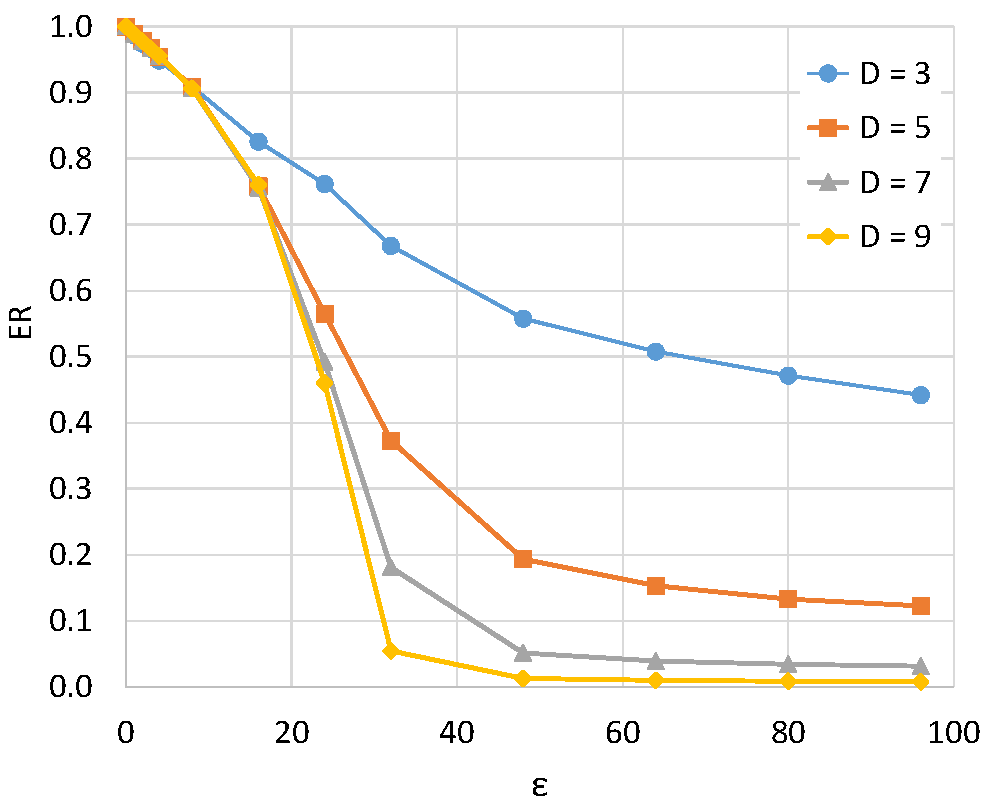
\includegraphics[width=5cm]{Figures/Random_Trees_BAB_depth2_er.pdf} }}%
    \hfill
    \subfloat[$\amb$ as a function on $\epsilon$]{{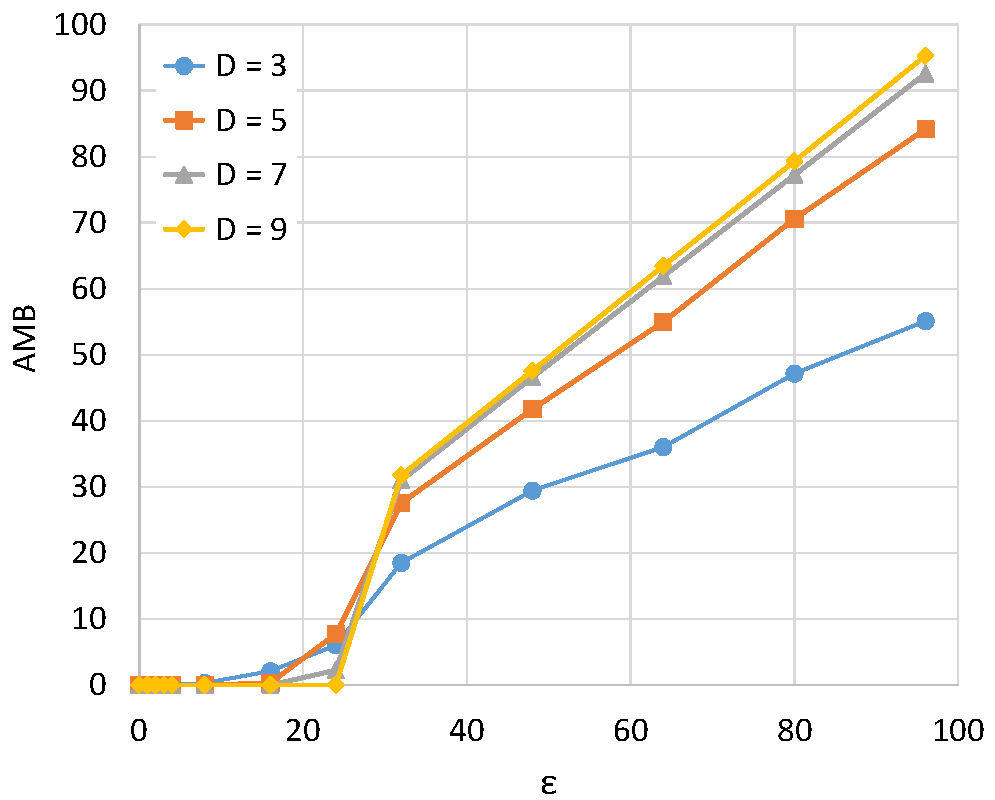
\includegraphics[width=5cm]{Figures/Random_Trees_BAB_depth2_amb.pdf} }}%
    \hfill
    \subfloat[$\amb$ as a function on $\er$ bins.]{{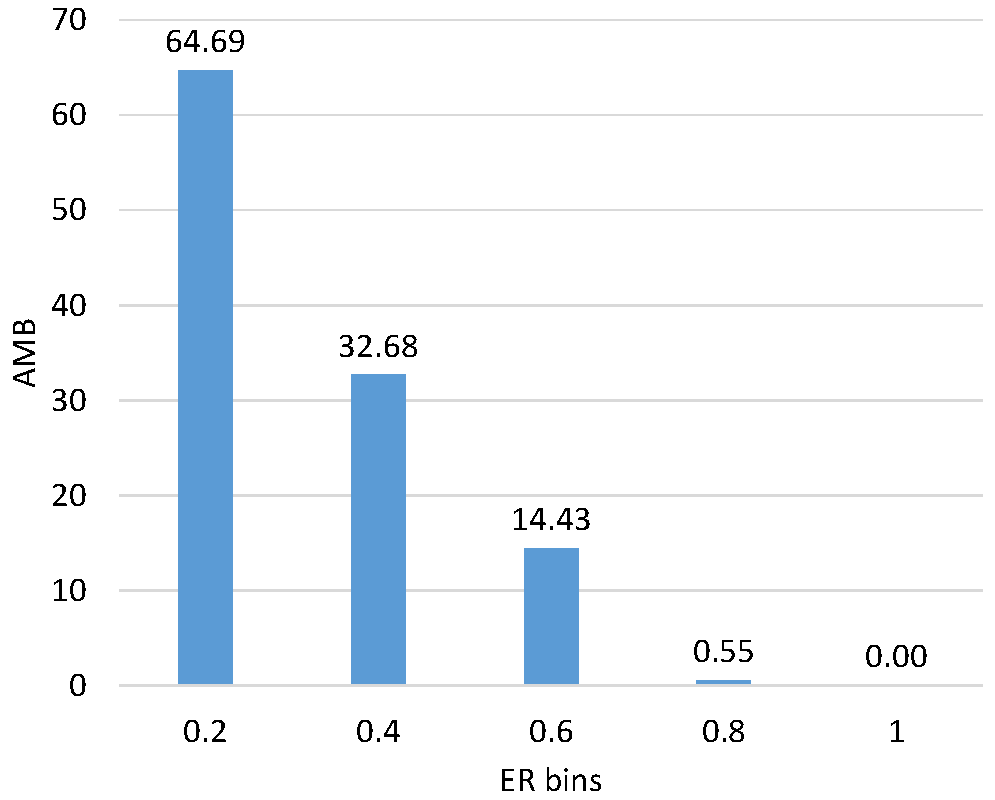
\includegraphics[width=5cm]{Figures/Random_Trees_BAB_depth2_bins.pdf} }}%    
    \caption{Experimental results for the deterministic RT domain.}%
    \label{fig:exp-rt-det}%
\end{figure*}



%\begin{figure}
%	\centering
%	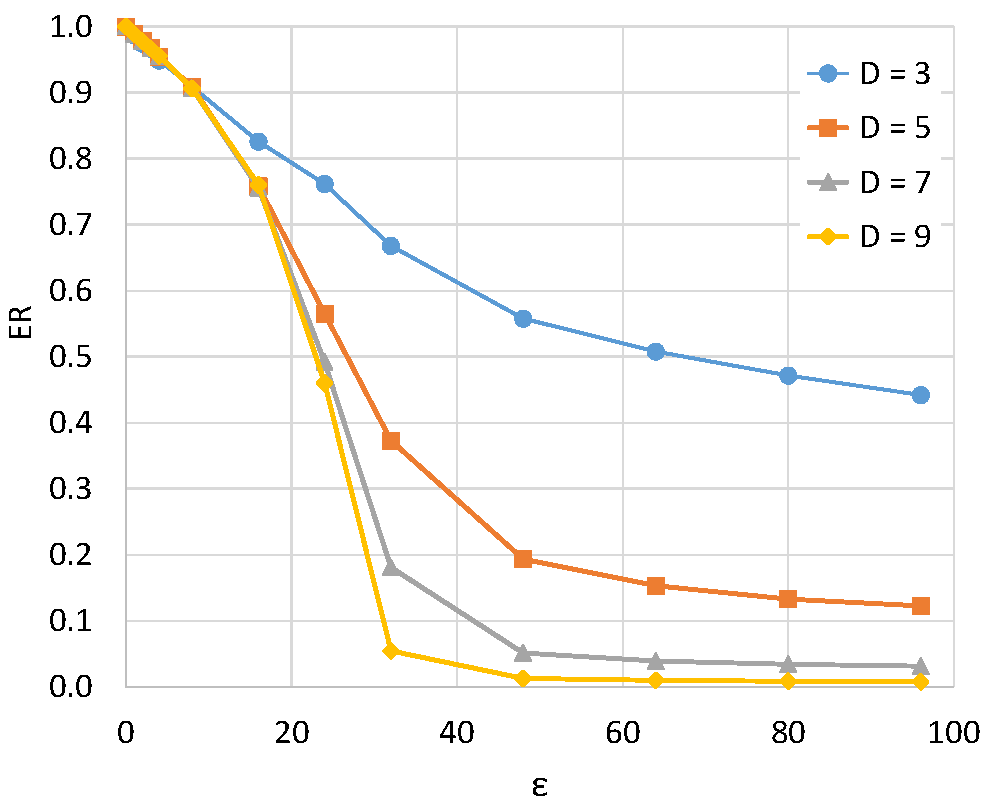
\includegraphics[width=0.8\columnwidth]{Figures/Random_Trees_BAB_depth2_er.pdf}
%	\caption{Deterministic RT domain. Comparing $\er$ as a function on $\epsilon$.}
%	\label{fig:exp-random2}
%\end{figure}

%\begin{figure}
%	\centering
%	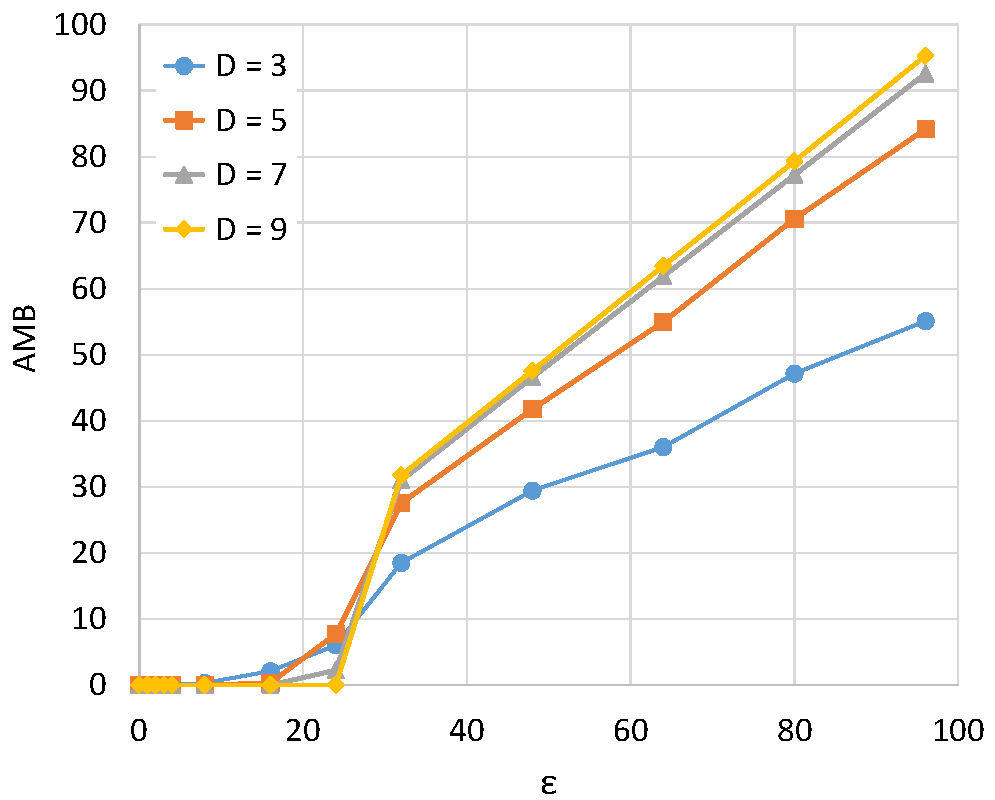
\includegraphics[width=0.8\columnwidth]{Figures/Random_Trees_BAB_depth2_amb.pdf}
%	\caption{Deterministic RT domain. Comparing $\amb$ as a function on $\epsilon$.}
%	\label{fig:exp-random1}
%\end{figure}

%\begin{figure}
%	\centering
%	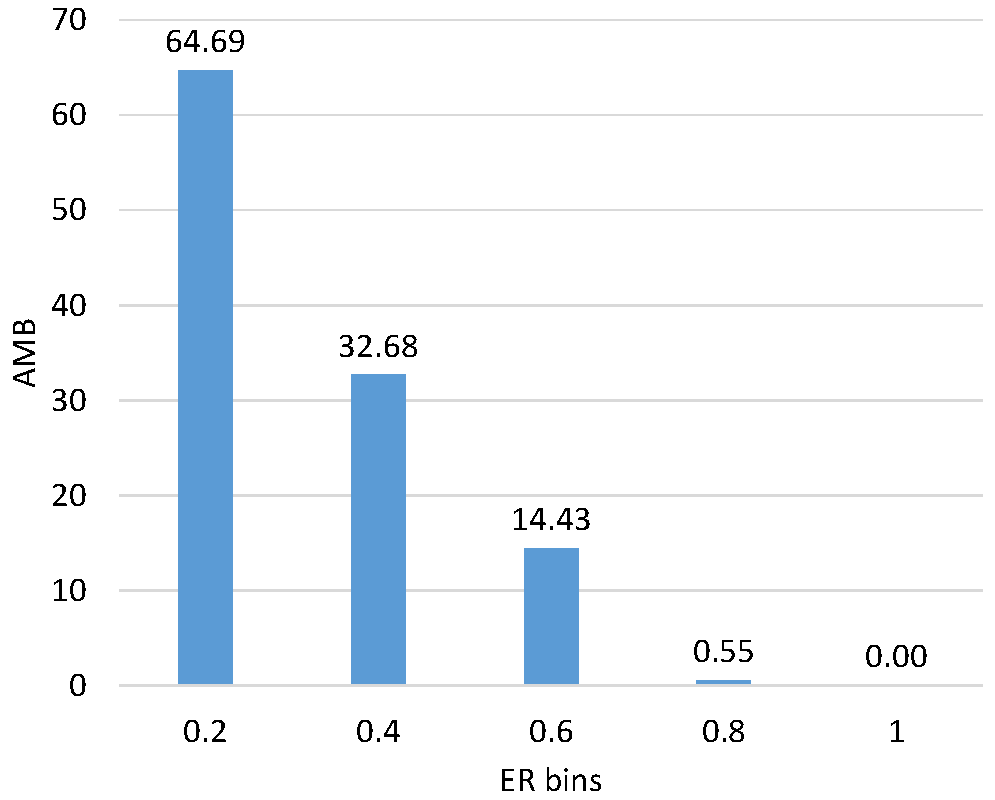
\includegraphics[width=0.8\columnwidth]{Figures/Random_Trees_BAB_depth2_bins.pdf}
%	\caption{Deterministic RT domain. Comparing $\amb$ as a function on $\er$ bins.}
%	\label{fig:exp-random3}
%\end{figure}


Figure \ref{fig:exp-rt-det}(a) shows the average $\er$ as a function of $\epsilon$ for RT instances with branching factor of 4 and depths of $3$, $5$, $7$, and $9$.
Each data point is an average over 50 instances. 
As expected, increasing $\epsilon$ decreases the $\er$ value, as more pruning occurs and consequently less nodes are being expanded.
In addition, the impact of our bounded pruning increases for larger game trees: running BAB with the same $\epsilon$ for deeper trees yielded a smaller $\er$.
This occurs because increasing the size of the game tree creates larger sub-trees that can be exploited by BAB and get pruned. 

Figure \ref{fig:exp-rt-det}(b) shows the average $\amb$ as a function of the $\epsilon$ over the same instances. As can be seen, for all depths, as we increase the $\epsilon$ value, the $\amb$ is increased as well, but never beyond $\epsilon$, as expected. For example for depth of 9, the $\amb$ for $\epsilon=0$ is zero, the $\amb$ for $\epsilon=32$ is 30.97, and the $\amb$ for $\epsilon=64$ is 61.88. 

%[[Roni: (1) From the figure, I can't see these values of epsilon since they are too small. I recommend showing these results in a table. (2) Do not show the trend only on epsilon=0 and another value, since epsilon=0 is just safe pruning, e.g., show epsilon=0 and 128]] 
The impact of the depth of the tree on the average $\amb$ is not as dramatic as on the average $\er$.
Still, the $\amb$ for deeper trees is clearly larger, for the same value of $\epsilon$, than for shallower trees.
For example for $\epsilon$ of 32, for depth of 3, 5, 7, and 9, the $\er$ is 0.67, 0.37, 0.18, and 0.05, respectively.
%[[Roni: Dor, add a specific example | Dor: I added]]. 
This trend can be explained by the fact that increasing the size of the tree creates more pruning opportunities, and consequently more opportunities to increase the minimax bound. 
%[[Roni: Last argument is not super strong]]
Figure~\ref{fig:exp-rt-det}(c) shows the relation between the $\er$ and $\amb$ values.
Here, we divided all instances with branching factor of 4 and depth of 5, into 5 bins.
The first bin calculate the average over all instances with $\er$ of $0$ to $0.2$, the second bin over $\er$ of $0.2$ to $0.4$ and so on.
It is easy to see that smaller $\er$ correspond with larger $\amb$, as expected, extensive pruning causes smaller $\er$ and wider gap between the values of the $\pess$ and the $\opti$.
Same trend was observed in all couples of branching factor and depth that we tested. 


\begin{figure*}[t]
    \centering
    \subfloat[$\er$ as a function on $\epsilon$]{{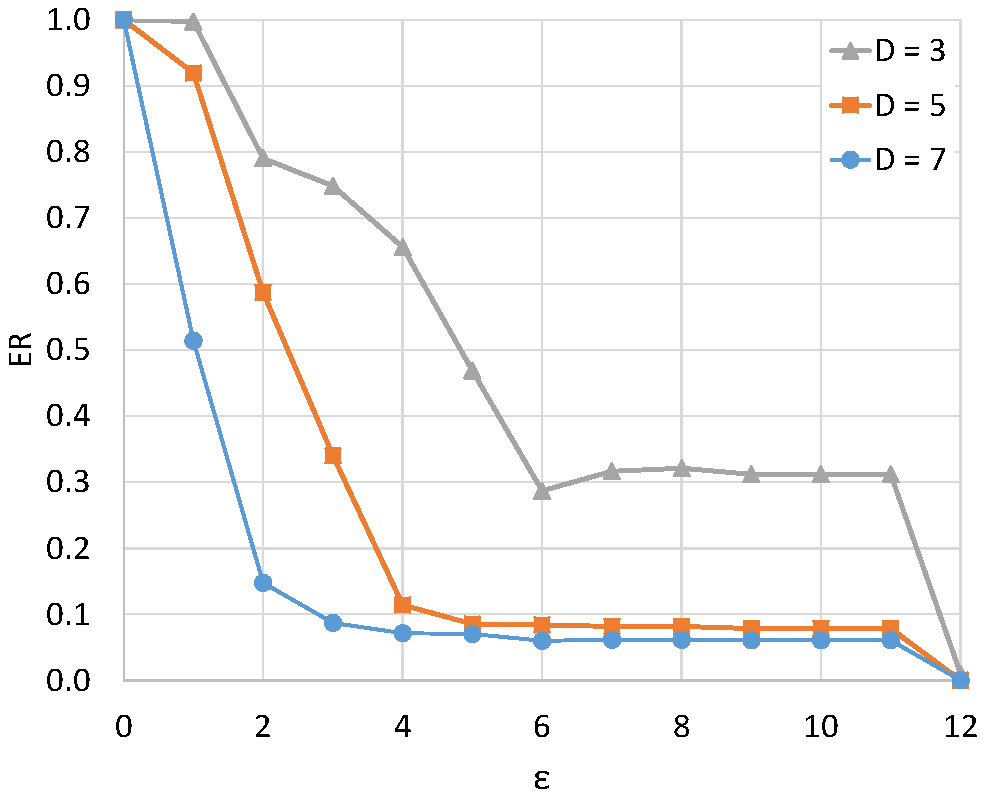
\includegraphics[width=4.75cm]{Figures/Cops_And_Robber_BAB_depth3_er.pdf} }}%
    \hfill
    \subfloat[$\amb$ as a function on $\epsilon$]{{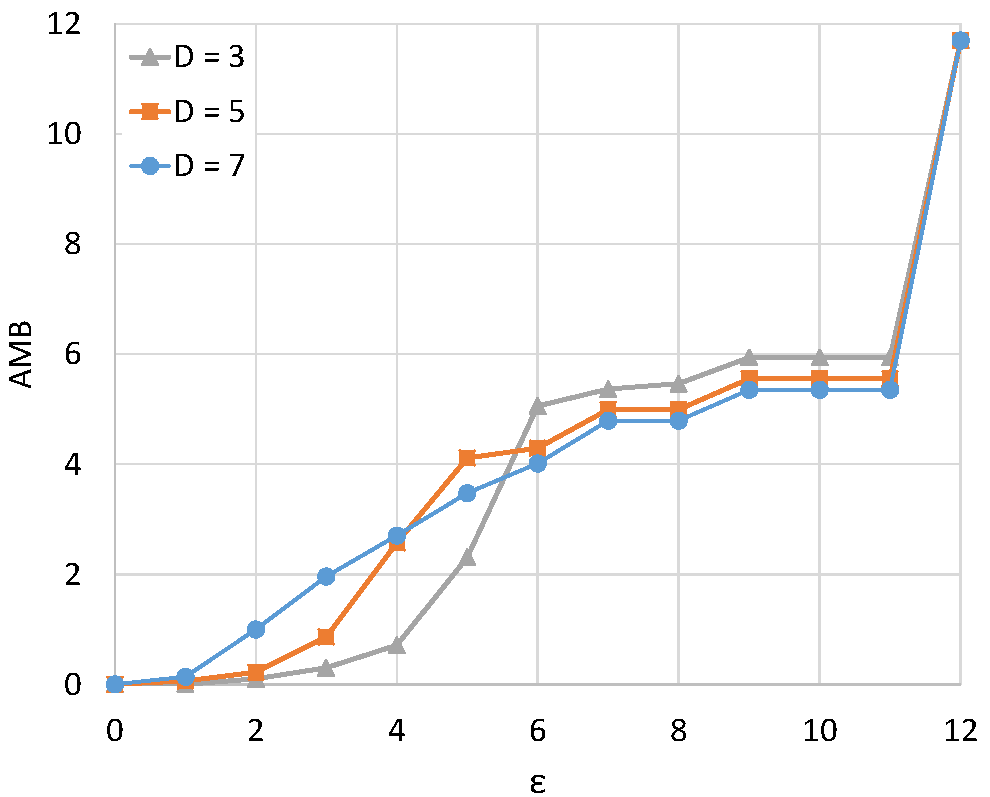
\includegraphics[width=4.75cm]{Figures/Cops_And_Robber_BAB_depth3_amb.pdf} }}%
    \hfill
    \subfloat[$\amb$ as a function on $\er$ bins.]{{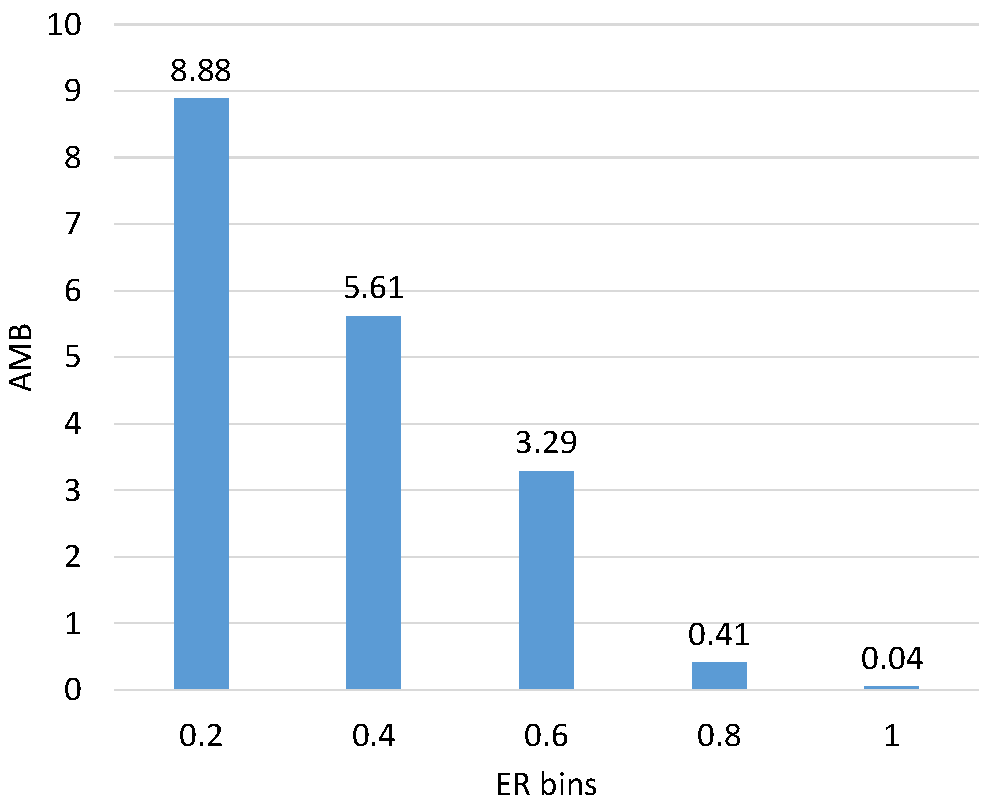
\includegraphics[width=4.75cm]{Figures/Cops_And_Robber_BAB_depth3_bins.pdf} }}%    
    \caption{Experimental results for the deterministic C\&R domain.}%
    \label{fig:exp-cr-det}%
\end{figure*}



%\begin{figure}
%	\centering
%	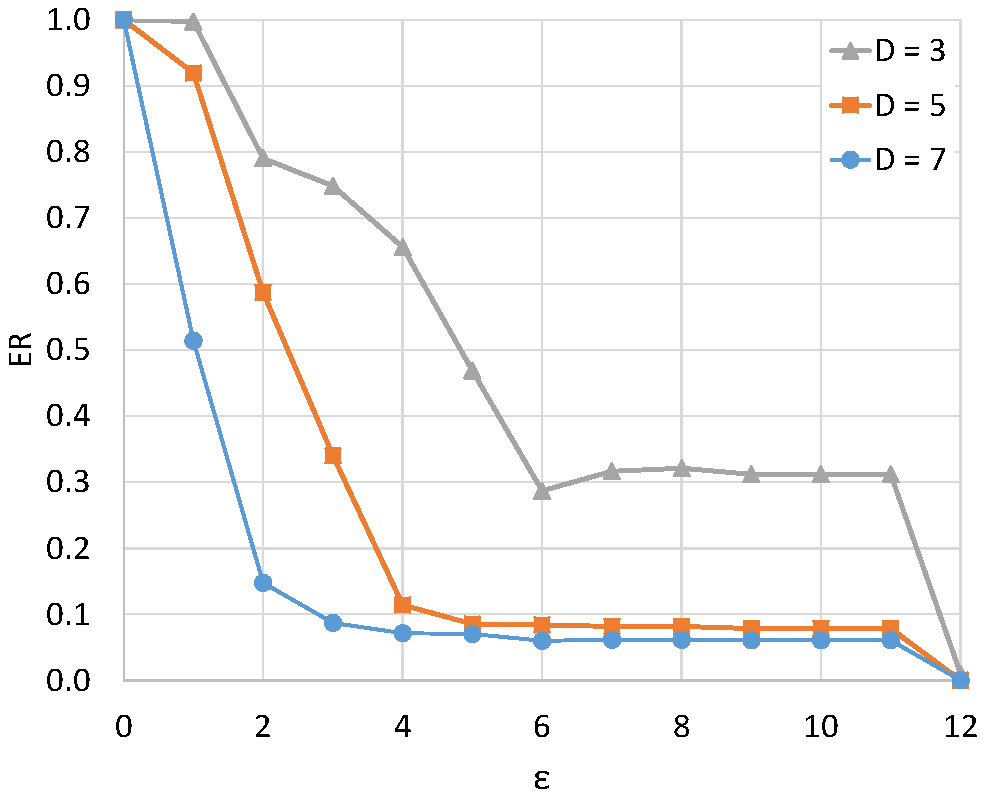
\includegraphics[width=0.8\columnwidth]{Figures/Cops_And_Robber_BAB_depth3_er.pdf}
%	\caption{Deterministic C\&R domain. Comparing $\er$ as a function on $\epsilon$.}
%	\label{fig:exp-car2}
%\end{figure}
%\begin{figure}
%	\centering
%	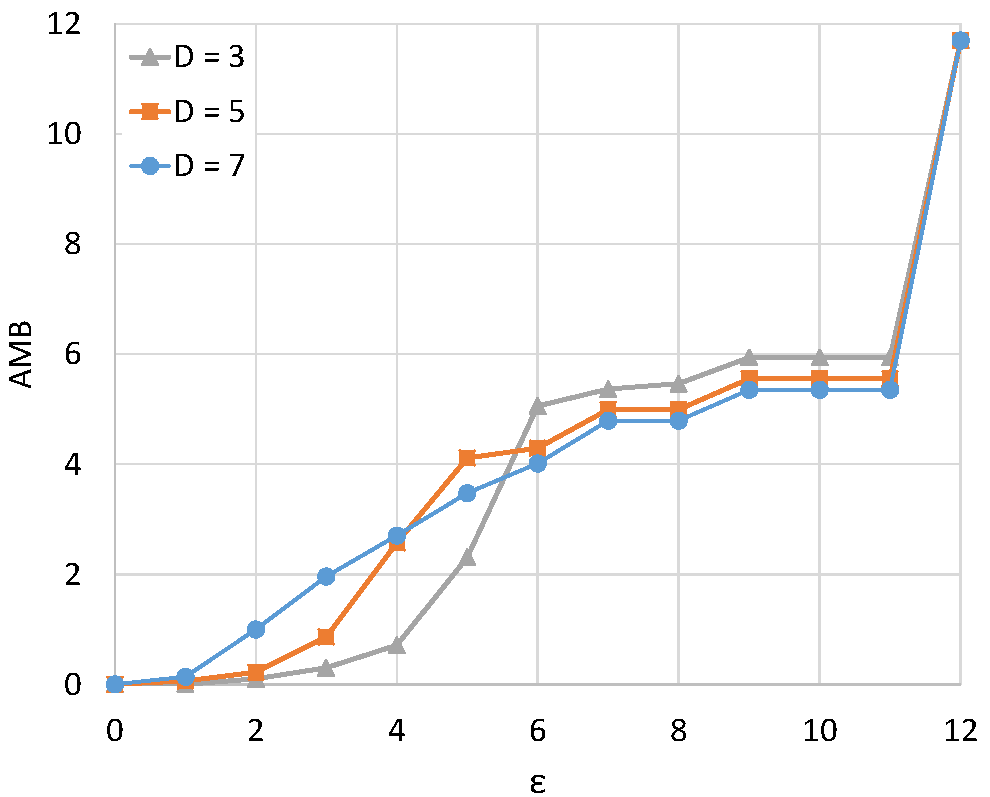
\includegraphics[width=0.8\columnwidth]{Figures/Cops_And_Robber_BAB_depth3_amb.pdf}
%   \caption{Deterministic C\&R domain. Comparing $\amb$ as a function on $\epsilon$.}
%	\label{fig:exp-car1}
%\end{figure}
%\begin{figure}
%	\centering
%	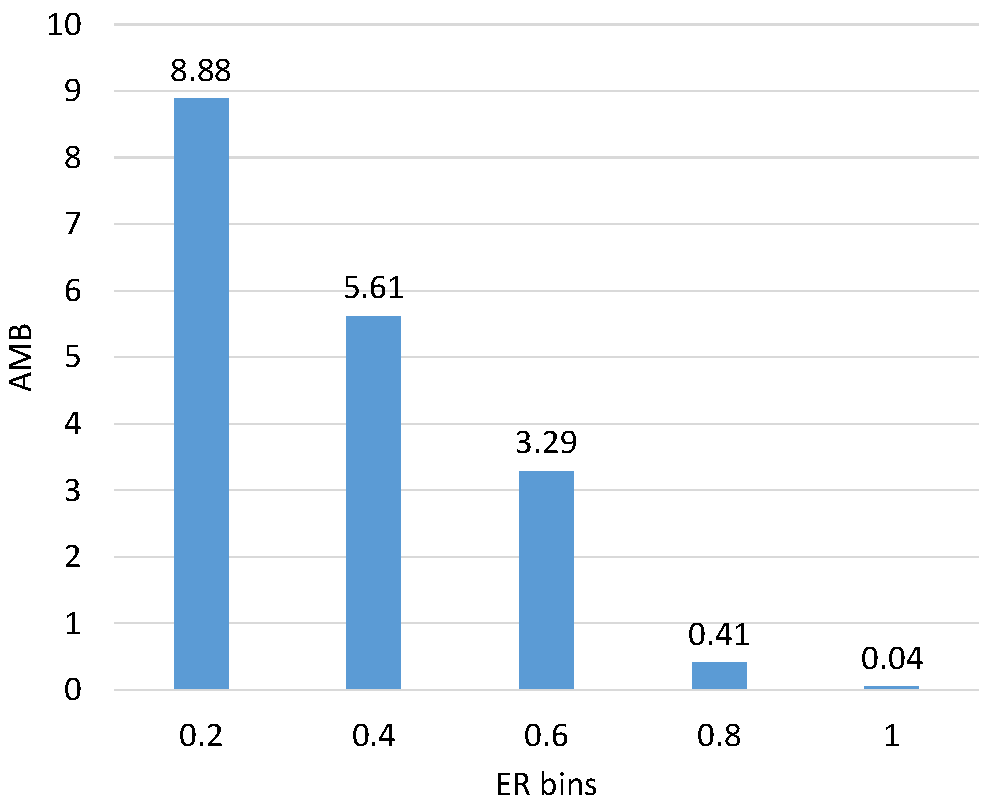
\includegraphics[width=0.8\columnwidth]{Figures/Cops_And_Robber_BAB_depth3_bins.pdf}
%    \caption{Deterministic C\&R domain. Comparing $\amb$ as a function on $\er$ bins.}
%	\label{fig:exp-car3}
%\end{figure}

Figures \ref{fig:exp-cr-det}(a) and (b) show the average $\er$ and $\amb$, respectively, as a function of  $\epsilon$ for 50 random instances of the C\&R game on 6$\times$6 open grid with 3 cops and depths of $3$, $5$, and $7$. Here, $\vmin=0$ and $\vmax=12$. The cops can not catch the robber before $\vmin=0$ because here the score is the time in which the cops catch the robber, and $\vmax=12$ is the maximum manhattan distance of the grid.
%[[Roni: Dor, any hint on how you got to these numbers? | Dor: I wrote something about it]] 
Here too, we see that increasing $\epsilon$ results in lower $\er$ and higher $\amb$, as expected. Also, we see the same trend with the impact of the depth of the tree on the average $\er$, however the impact of the depth  on the average $\amb$
here is not as conclusive. \ref{fig:exp-cr-det}(c) shows the same division of all instances with depth 3 into bins as in figure~\ref{fig:exp-rt-det}(c) and the same trend that observed in previous experiment. 

%---------------------------------------------------------
\subsection{Games with Chance}

%\subsubsection{Domains}
%\subsubsection{Results}

\begin{figure*}[t]%
    \centering
    \subfloat[$\er$ as a function on $\epsilon$]{{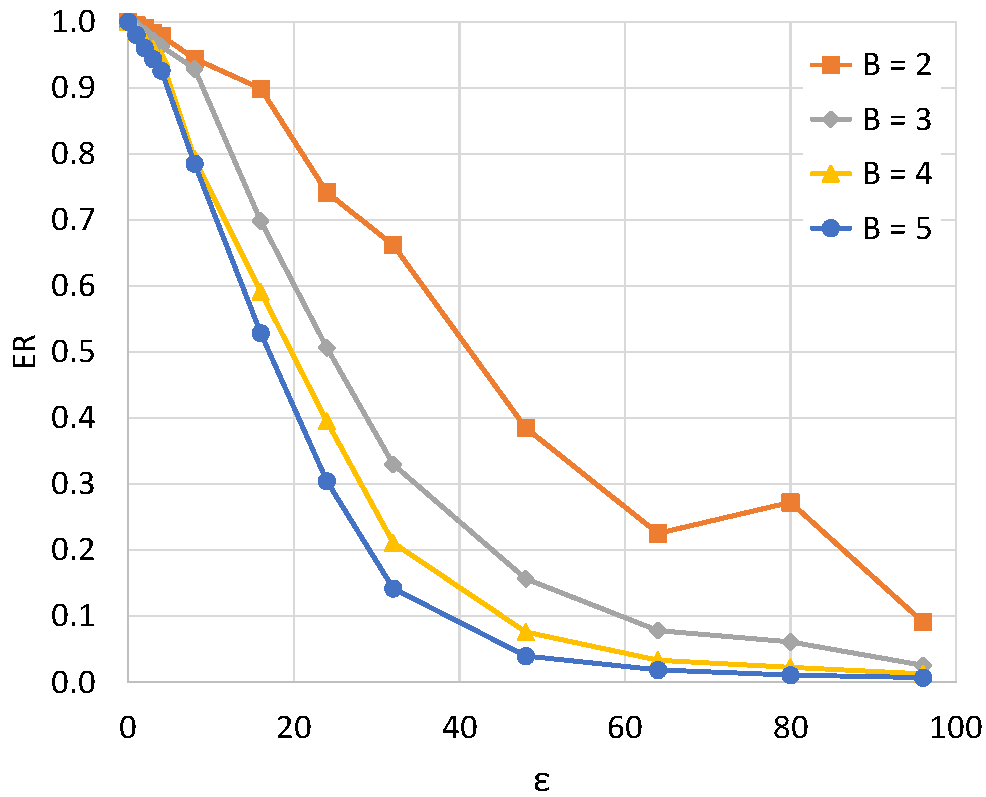
\includegraphics[width=4cm]{Figures/Random_Trees_BAB_depth_chance2_er.pdf} }}%
    \hfill
    \subfloat[$\amb$ as a function on $\epsilon$]{{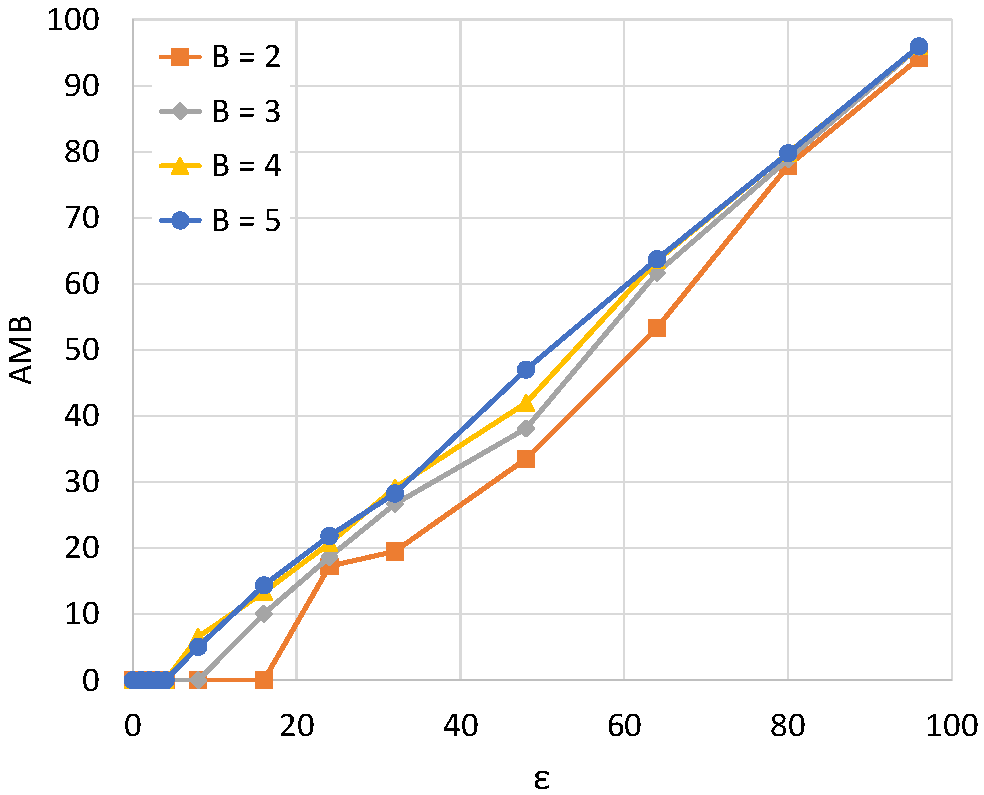
\includegraphics[width=4cm]{Figures/Random_Trees_BAB_depth_chance2_amb.pdf} }}%
    \hfill
    \subfloat[$\er$ as a function on $\epsilon$]{{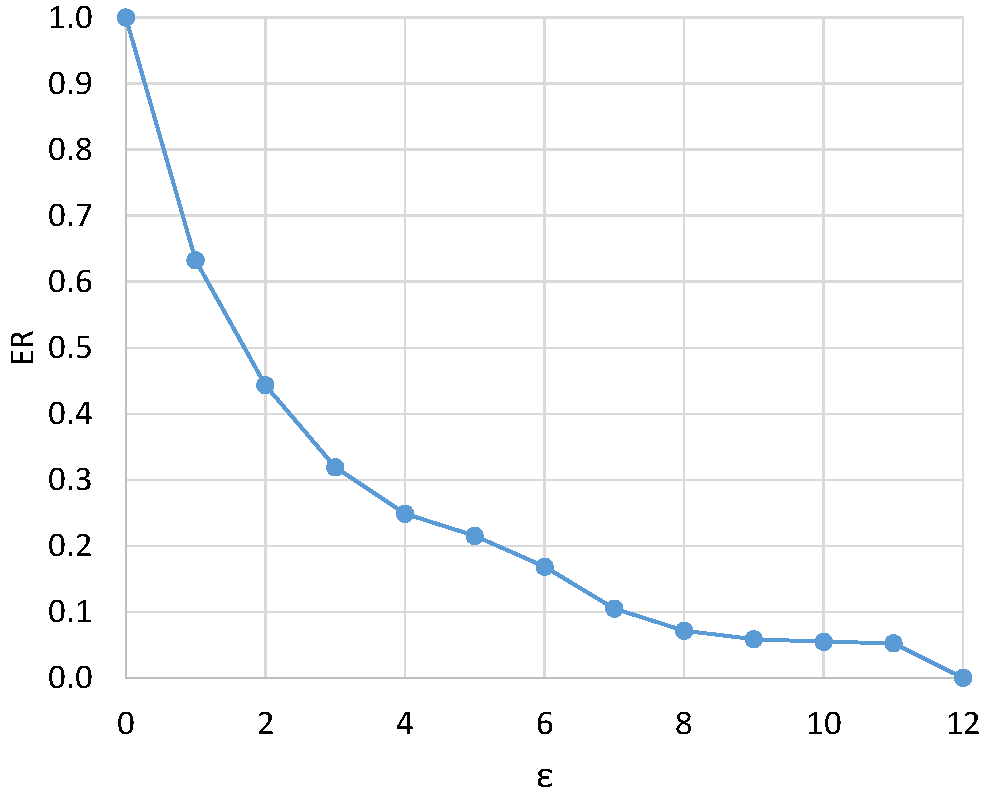
\includegraphics[width=4cm]{Figures/Cops_And_Robber_BAB_depth_chance3_er.pdf} }}%
    \hfill
    \subfloat[$\amb$ as a function on $\epsilon$]{{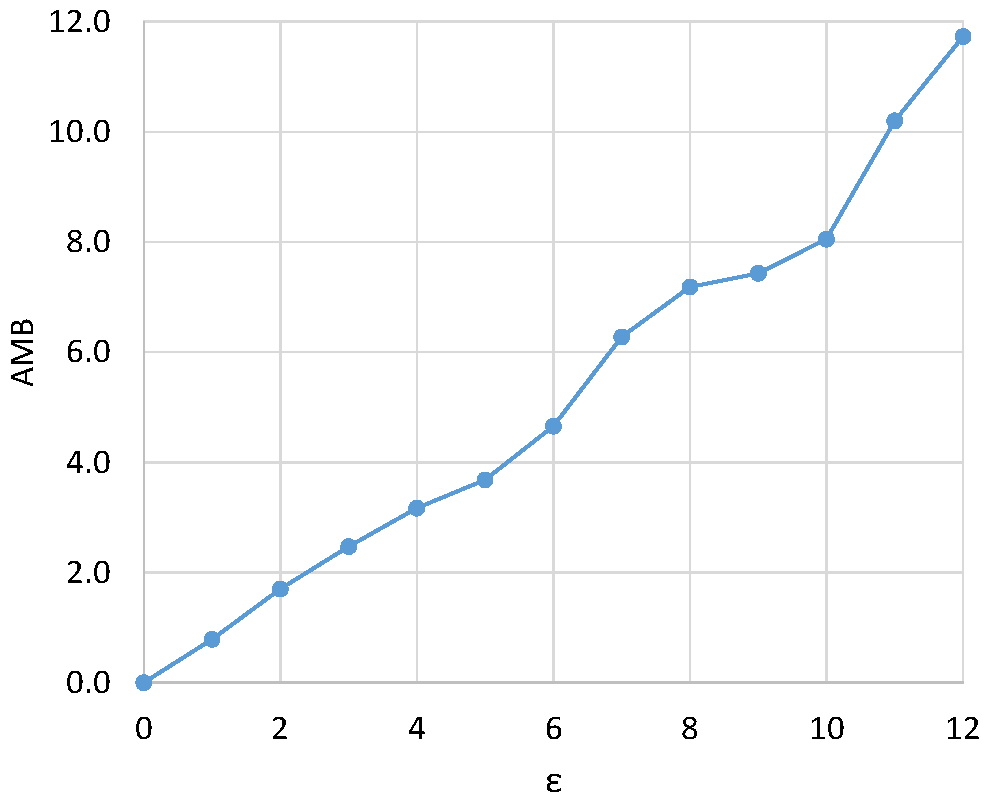
\includegraphics[width=4cm]{Figures/Cops_And_Robber_BAB_depth_chance3_amb.pdf} }}%
    \caption{Experiments on domains with chance.}
	\label{fig:exp-chance}
\end{figure*}




%The random trees can also contain a stochastic element. We created random trees where after each player turn the selected move occurs in probability $p$ and each of the unchosen moves occurs in probability $\frac{1-p}{b-1}$. 
Figures~\ref{fig:exp-chance}(a) and (b) show the average $\er$ and $\amb$, respectively, as a function of $\epsilon$ for 50 random instances of stochastic RT, for depth=$4$ and branching factor of $2$, $3$, $4$, and $5$. Again, the general trend in which higher $\epsilon$ corresponds to lower $\er$ and higher $\amb$ is clearly observed. For example for branching factor of 4, for $\epsilon$ of 0, 8, and 24, the $\er$ is 1, 0.79, and 0.4, respectively, and the $\amb$ is 0, 6.58, and 20.71, respectively.
%[[Roni: Dor, please add concrete example of one data point. This helps reader to follow | Dor: added]]. 
Note that for the specific case of $\epsilon=80$ and branching factor=2 there is a slight increase in $\er$ compared to $\epsilon=60$. Such rare events are possible, as shown in Figure~\ref{fig:bab-prune}. 
Consider now the effect of increasing the branching factor. The results show that increasing the branching factor for the same $\epsilon$ are in general that higher branching factor corresponds to lower $\er$ and higher $\amb$. The reason is similar to the explanation of how depth impacted $\er$ and $\amb$ in the deterministic case: larger branching factor corresponds to larger tree allowing more pruning opportunities. 
In fact, we experimented with different branching factor and tree depth in both deterministic and stochastic cases and observed these trends in both setting. 
%[[Roni: Dor, please verify that this is indeed correct. I am almost certain this is what we've seen, but please verify| Dor: It is correct, I just checked]] 
%Here also we divided all the instances with branching factor of 4 and depth of 4 by the $\er$ into bins in figure~\ref{fig:exp-random3}, as done in the two experiments above, and here also we can observe the same trend. 

Finally, Figures~\ref{fig:exp-chance}(c) and (d) show the average $\er$ and $\amb$, respectively, as a function of $\epsilon$ for 50 random instances of the C\&R game with chance on 6x6 grid with 20\% randomly allocated obstacles, 3 cops, $\vmin=0$, $\vmax=12$, and depth=$3$.\footnote{We experimented with a wide range of parameters and settings, and show this setting as a representative example.} Here too we see the same general trends: higher $\epsilon$ yields lower $\er$ and higher $\amb$. For example, for $\epsilon$ of $0$, $4$, and $8$, the $er$ is $1$, $0.25$, and $0.07$, respectively, and the $\amb$ is $0$, $3.17$, and $7.19$, respectively.
%Figure \ref{fig:exp-car-chance3}, as was done in all previous experiments, shows a division of $\er$ into 5 bins and maintains the relation between the $\er$ and the $\amb$  as in the other equivalent experiments.
%[[Roni: Dor add a concrete example | Dor:done]].
%[[Roni: Dor, if we did not see the depth and branchign factor effects here, please add a sentence saying this. I think we did not see these trends, so important to let the world know]]

%---------------------------------------------------------
%---------------------------------------------------------
\section{Related Work}

There is a large volume of literature on Alpha-Beta and *-Minimax variants and improvements. 
Work on bounding the minimax value dates back to Pearl's SCOUT algorithm (\citeyear{pearl1980scout}) or even earlier. The main concept used by most such methods is to initialize $\alpha$ and $\beta$ by some values that are different from $\vmin$ and $\vmax$, providing stronger pruning. 
The range between these initial values is called the Alpha Beta window. If the minimax value is not withing the Alpha Beta window, the search fails. Some algorithms, e.g., Nega Scout~\cite{reinefeld1983improvement}, follow with this approach and perform multiple calls to Alpha Beta with different windows. 
In general, these algorithms either find the minimax value or fail (high or low). By contrast, a bounded-suboptimal algorithm finds a solution that is within $\epsilon$ of the minimax value. %S requirement, since without knowing the minimax value one cannot know how to set the Alpha Beta window  relate the desired sub optimality $\epsilon$ to the reinefeld1983improvement
%[[TODO: Mention alpha beta variants that do unsafe pruning, and windowed alpha beta]]

More recent work also studied improvements for *-Minimax for games with chance, including using transposition tables~\cite{veness2007effective}, and performing forward pruning~\cite{schadd2009chanceprobcut}. While the latter also does pruning as we do, it does not provide the suboptimality guarantee that we do. 

\section{Conclusion, Discussion, and Future Work}
In this work, we proposed the concept of a bounded-suboptimal algorithm for game tree search, as a way for approximately solving two player zero-sum games with full observability. The theoretical framework for building such algorithms is given for games with and without chance, and a concrete bounded-suboptimal algorithm is presented called Bounded Alpha-Beta (BAB). Experimental results on two domains confirm that BAB can tradeoff solution quality for runtime effectively. 


This work opens a wide range of directions for future work on bounded suboptimal game tree search. 

\noindent {\bf Different game tree search strategies.} Our algorithm is based on classical Alpha-Beta and its extension to games of chance, but Theorem~\ref{the:basic} applies directly to any other game tree search algorithms, including Monte Carlo Tree Search solver~\cite{lanctot2013monte} and Proof Number Search~\cite{allis1994proof}. Exploring how suboptimal-bounding affects their behavior. 

%Also, our analysis shows that in games of chance there is more flexibility than we currently exploit, by allowing re-distributing the desired suboptimality bound in different ways between the children of chance nodes. These are exciting topic for future work. Also, while this work has focused on finding a minimax-bound and \emph{solving} the game, future work will investigate how our results can be used for developing \emph{game playing} algorithms. 

%\subsubsection{Redistributing $\epsilon$}
%Line~\ref{line:zeta} in Algorithm~\ref{alg:weightedAlphaBeta} is the recursive call for computing $\opti$ and $\pess$ of the child of the current node. 
\noindent \textbf{Dynamic suboptimality bound.}
A deeper look on the proof of Theorem~\ref{the:basic} reveals that it is possible to have more flexibility in how $\epsilon$ is distributed between the children of a CHANCE node. Instead of passing $\epsilon(n)$ to each child node $c$, it is possible to provide different values of $\epsilon$ to different children of $n$. 
Let $\epsilon(c)$ be the $\epsilon$ passed to a child node $c$ in line~\ref{line:recursive} in Algorithm~\ref{alg:weightedAlphaBeta}. The following relation between $\epsilon(n)$ and $\epsilon(c)$ is sufficient to maintain the desired suboptimality. 
\begin{equation}
  \sum_{c\in C(n)} \epsilon(c) \pi(c) \leq \epsilon(n) \label{eq:redistribute}
\end{equation}
%	and all the conditions specified in Theorem~\ref{the:basic} hold then 
%	$\MM(\rootnode)\in    [\pess(\rootnode),\pess(\rootnode)+\epsilon]$
%The following condition is sufficient to maintain the  guarantee provided by Theorem~\ref{the:basic}  
%Instead of running each child of a chance node with the same $\epsilon$, one can use different values of $\epsilon$ for the there is a recursive call for 
%\begin{theorem}
%	\label{theorem_error_bound}
%	If for every CHANCE node $n$ it holds that
%	\[ \sum_{c\in C(n)}
%			\epsilon(n) \leq \epsilon(n) \]
%	and all the conditions specified in Theorem~\ref{the:basic} hold then 
%	$\MM(\rootnode)\in
 %   [\pess(\rootnode),\pess(\rootnode)+\epsilon]$
%\end{theorem}
Future work will investigate how to distribute  $\epsilon$ to the children of CHANCE nodes according to Eq.~\eqref{eq:redistribute} to allow further pruning and faster search. 

\noindent \textbf{Game playing with BAB.} We performed a very preliminary set of experiments to investigate how a player using BAB with $\epsilon>0$ fares against Alpha Beta, which is equivalent to BAB with $\epsilon=0$.
We experimented on the deterministic version of C\&R with 3 cops and a 6$\times$6 grid and $\epsilon$ values of 0, 1, 2, 4, and 8. We limited the number of node expansions allowed in each step to 200,000, and had each algorithm run in an iterative deepening manner until the the total number of node expansions exceeded 200,000, choosing the  best move according to the last iteration.
Each instance played twice, once with each starting player, and a player is determined as a winner if its average score over the two games is greater than the other's.
The results showed that BAB with $\epsilon=1$ won 11 times, lost 6 times, and had a draw 33 times, but BAB with $\epsilon=2$ it won 6 times, lost 12 times, and had a draw 32 times.
This shows some potential for BAB but further research is needed. 

\noindent \textbf{$\epsilon$-equilibrium.} 
The optimal policy for MAX and MIN players that use classical Alpha-Beta pruning is known to be a Nash equilibrium, that is, no player can gain by unilaterally deviating from its action. Obviously, a the policy proposed in~"\ref{sec:bab}" section obtained by BAB in not necessarily a Nash equilibrium. However, we conjecture that this policy reaches an  $\epsilon$-equilibrium~\cite{nisan2007algorithmic}, which is a joint policy in which no player can gain more than $\epsilon$ by unilaterally deviating from his strategy. Proving this conjecture is a topic for future research.





\section{Acknowledgements}
This research was supported by the Israel Ministry of Science, the Czech Ministry of Education, and by ISF grant \#210/17 to Roni Stern.

\bibliography{games}
\bibliographystyle{aaai}
\end{document}


